





\begin{comment}
    
    THINGS TO MENTION
    
    
     --- PAPER pizzati+20 CAREFUL DESCRIPTION
    
     --- f\_esc DEPENDENCE CAREFUL CALCULATION FOR DUST AND DESCRIBE THE ROLE OF FESC IN REIONIZATION AND ATTEMPTS TO MEASURE ITS VALUE
     
     
     --- METALLLICITY DEPENDENCE SEE REVIEW RESPONSE
 
\end{comment}



In the last chapter, we have concluded that outflows are the most promising candidate to explain the presence of extended \CII halos in high-z galaxies. However, this conclusion was solely based on very general theoretical considerations, on few observations hinting at a correlation between outflows and extended \CII emission, and -- above all -- on the presence of arguments that disfavored all the other possible solutions. Moreover, as already pointed out, even the \textit{outflows hypothesis} struggles to explain the formation of extended \CII halos in numerical simulations that include the presence of stellar feedback in the form of galactic winds. For these reasons, the problem of \CII halos formation is yet to be solved. 

In the remaining part of this thesis, we elaborate on the outflow hypothesis by providing a semi-analytical model for a galactic wind that is able to account for the \CII emission revealed by observations. Our model is founded on very simple but physically reasonable assumptions. Indeed, this simplicity is one of the strengths of our model, as it let us investigate in detail the physical processes that lead to the formation of \CII halos and infer some interesting conclusions on the physical environment where these halos arise. However, our semi-analytical approach has some intrinsic limitations, as some of the assumptions on which it is based are somewhat arbitrary, and they need to be carefully assessed by detailed numerical studies. We will comment further on the strengths and weaknesses of our model in the conclusions of this work (chap. \ref{chap:conclusion}).

This chapter, instead, is devoted to a thorough description of the model, and to the analysis of the physical processes involved in the \CII emission. We will make use of many of the theoretical tools we have laid down in the first three chapters of this work. We start by refining these tools in the context of gas cooling and heating (section \ref{sec:gas_cooling_heating}). Then, we focus on the physical properties of our model (section \ref{sec:outflow_model}) by making use of the theory of galactic winds introduced in chapter \ref{chap:outflows}. We obtain radial profiles for the key thermodynamical variables, and we study the ionization state of the outflowing gas. This allows us to take the last step forward, and to compute the expected \CII emission from the wind (section \ref{sec:CII_emission}).


\section{Gas cooling and heating}\label{sec:gas_cooling_heating}


We have already discussed quite extensively the importance of cooling and heating processes in early galaxy evolution physics. These processes are in fact responsible for driving gas accretion from the hot virialized halo into the inner regions of the galaxy (section \ref{sec:accretion}), and they may come into play in feedback processes as well (section \ref{sec:outflows_cooling}). More generally, heating and cooling play a key role in determining the physical conditions of the gas both in the ISM/CGM of galaxies and in the external IGM. 

In this section, we describe heating and cooling processes that are important in determining the state of gas in astrophysical systems. This discussion is relevant to our work, as cooling/heating of outflowing gas will form the basis of our model in section \ref{sec:model_outflows}. 

\subsection{Cooling mechanisms}\label{sec:cooling}

We start by considering the cooling of a gas in a general astrophysical environment. As already mentioned, a gas cools by emitting radiation, and thus losing part of its thermal energy. In order to describe this process, we have to introduce some basic concepts of light-matter interaction theory.

Let us focus on an atomic gas of a given species $x$. Quantum mechanics predicts that electrons of a given atom can occupy a set of atomic levels at fixed energies ${E_i}$. Interacting with an electromagnetic field, an electron can transition between a level $i$ and a level $j$. Three types of transitions are possible: \textit{absorption}, \textit{stimulated emission}, and \textit{spontaneous emission}. In an absorption process from the level $i$ to the level $j$ (w.l.o.g., $j>i$), an incident photon with energy $h\nu_{ij}=E_j-E_i$ is absorbed by an electron, and it causes the electron to jump to the level $j$. 

Using time-dependent perturbation theory, it can be proven that the rate (i.e., the number of events per unit time) of transition due to absorption is $\mathcal{R}_{ij} = B_{ij} I(\nu_{ij})$, where $I(\nu_{ij})$ is the intensity of the electromagnetic field at the frequency of transition and $B_{ij}$ is a coefficient describing the strength of the transition. Similarly, in the stimulated emission mechanism, the electron is initially on level $j$, but the interaction with the incident photon causes the electron to jump down to the level $i$, emitting a photon that is perfectly identical to the incident one. Also in this case, the rate has the same form, although the coefficient is different: $\mathcal{R}_{ji}^{(1)} = B_{ji} I(\nu_{ji})$. 

Spontaneous emission works differently, as no incident radiation is present, but a level-$j$ electron can spontaneously emit radiation transitioning down to level $i$. The rate for this process is defined using a third coefficient: $\mathcal{R}_{ji}^{(2)} = A_{ji}$. The three coefficients $B_{ij}$, $B_{ji}$, and $A_{ji}$ are known as \textit{Einstein coefficients}. They are connected by a set of relations:
\begin{subequations}
\begin{align}
    &g_i\,B_{ij} = g_j\,B_{ji}\\
    &A_{ji} = \frac{2h\nu_{ij}^3}{c^2}\,B_{ji},
\end{align}
\label{eq:einstein_coeff}
\end{subequations}
where $g_i$ and $g_j$ are the statistical weights (i.e., the degeneracies) of the two levels. 

Therefore, it suffices to know one single coefficient to find the other ones. It is customary to express the $B_{ij}$ coefficient in terms of a dimensionless number, the oscillator strength $f_{ji}$:
\begin{align}
    B_{ji} = \frac{4\pi}{h\nu_{ji}}\,\frac{\pi e}{m_e c} \,f_{ji} 
\end{align}
$f_{ij}$ is essentially the effective number of classical oscillators involved in the transition. This number depends on the transition: different levels, in fact, can be connected by different kinds of transition, as the electromagnetic field interacts with electrons in different ways. At the first order, "electric dipole transitions" result from the interaction between the field and electrons. These transitions usually have an oscillator strength of the order of unity. 

If the dipole associated with the transition is zero, however, then higher-order terms become relevant: they are the "magnetic dipole" and "electric quadrupole" (the so-called "\textit{forbidden transitions}"). As they arise from the first order of the field expansion, the oscillator strength of these transitions is much smaller ($f\sim10^{-5}-10^{-8}$). 

As an aside, we note here that a similar discussion is valid for more complex systems such as molecules. The main difference resides in the presence of new degrees of freedom (rotational and vibrational), that create new energy levels and therefore allow for a whole new set of transitions. The oscillator strengths for transition between vibrational and rotational levels are around $f\sim 10^{-5}-10^{-6}$.

Given these premises, we can get some insight into how a gas emits radiation by addressing a simplified setting with a two-level atomic system. Generalizing this setting to the cases of interest will be pretty straightforward. We thus consider an upper level $u$ and a lower level $l$ separated by an energy gap $E_{ul}$. Under the hypothesis of statistical equilibrium, the rate of excitations from $l$ to $u$ equals the rate of de-excitations from $u$ to $l$. If no incident radiation is present, then transitions are induced by collisions and by spontaneous emission. Introducing the collisional rate coefficients, $\gamma_{lu}$ and $\gamma_{ul}$, we can write:
\begin{align}
    n_l \,n_x\,\gamma_{lu} = n_u\,n_x\,\gamma_{ul} + n_u\,A_{ul}, \label{eq:level_eq}
\end{align}
where $n_l$, $n_u$ are the densities of the lower and upper level respectively, while $n_x$ is the density of the species $x$ which is assumed to interact with the system through collisions. 

Because of detailed balance, the collisional rate coefficients of the two levels are
related via the relation ($g_{u,l}$ are the statistical weights of the two levels):
\begin{align}
    \gamma_{lu} = \frac{g_u}{g_l} \,\gamma_{ul}\,\exp(-E_{ul}/kT), \label{eq:coll_rates}
\end{align}
Using this condition, the statistical balance equation can be rewritten as:
\begin{align}
    \frac{n_u}{n_l} = \frac{g_u}{g_l}\,\frac{\exp(-E_{ul}/kT)}{1+n_{cr}/n_x}, \label{eq:level_population}
\end{align}
with the \textit{critical density}, $n_{cr}$, given by: $n_{cr} = A_{ul}/\gamma_{ul}$. This relation expresses the condition for Local Thermodynamic Equilibrium (LTE): if the density of the species $x$ is much larger than the critical density, then collisions dominate the de-excitation process, and thus we recover a level density that follows the Boltzmann equilibrium distribution. If, on the other hand, the density $n_x$ is smaller than $n_{cr}$, we are out of equilibrium, collisions are not frequent enough to populate the levels and most of the excited electrons will de-excite by spontaneously emitting a photon. We can quantify the distance of the system from thermodynamical equilibrium by introducing the \textit{excitation temperature} $T_\mathrm{exc}$:
\begin{align}
    kT_\mathrm{exc} = E_{ul}\log^{-1}\left(\frac{n_lg_u}{n_ug_l}\right) \label{eq:t_exc}
\end{align}
Using eq. \ref{eq:level_population}, we can connect the kinetic gas temperature with the excitation temperature using the following relation: 
\begin{align}
    \frac{T}{T_\mathrm{exc}} = 1 + \frac{kT}{E_{ul}}\, \log\left(1+\frac{n_{cr}}{n_x}\right)
\end{align}
As far as the density of the collisional partner is higher than $n_{cr}$, the excitation temperature is similar to the gas kinetic temperature. However, for smaller densities, $T_\mathrm{exc}$ gets significantly lower than the gas temperature, and this marks the exit from the equilibrium state. In astrophysical environments such as the ISM and the CGM/IGM, gas density is lower than the critical one for most of the species. This means that these systems are out of equilibrium, and in general, it is correct to focus on the low-density limit $n\ll n_{cr}$. 

The cooling law for this system can be obtained by noting that the energy per unit volume and time is simply given by the product of the spontaneous rate ($A_{ul}$) with the density of electrons in the upper level ($n_u$) and with the energy carried by every emitted photon ($h\nu_{ul}$). 

In this discussion, we are neglecting any effects of optical depth, by assuming that the gas is optically thin to radiation (i.e., photons emitted by the gas are never absorbed again and leave the system). This assumption holds true in many of the environments we are interested in, and it is coherent with our earlier assumption of no incident radiation. If the system were not optically thin, in fact, we would have to consider the effect that radiation emitted by the system itself has on the population of the two levels. 

In the optically thin limit, we can use eq. \ref{eq:level_population} as well as the conservation equation for the species $j$ ($n_u + n_l = \mathcal{A}_j n$, where $\mathcal{A}_j$ is the numerical abundance of the $j$ species in the gas and $n$ is the total gas density) to write:
\begin{align}
    n^2 \Lambda_j^{\mathrm{(cool)}} = n_u\,A_{ul}\,h\nu_{ul} = \frac{g_u/g_l\, \exp(-h\nu_{ul}/kT)}{1+n_{cr}/n_x+ g_u/g_l\, \exp(-h\nu_{ul}/kT)}\,\mathcal{A}_j\,n\,A_{ul}\,h\nu_{ul}
\end{align}
As already done in section \ref{sec:accretion}, we have expressed the energy lost by radiative cooling per unit time and volume $\dot{\varepsilon}$, as the product of the density squared with a \textit{cooling function} $\Lambda^{\mathrm{(cool)}}(T)$. The reason for this is clear by looking at the low density limit of the cooling law; if we take $n\ll n_{cr}$ and we use the definition of $n_{cr}$, then the cooling rate reads:
\begin{align}
    n^2 \Lambda_j^{\mathrm{(cool)}} \approx n_x \,n\, \mathcal{A}_j\,\gamma_{ul}\, h\nu_{ul}
\end{align}
This relation is simply stating that, as collisional de-excitation is inefficient, every upward collision results in a photon emitted spontaneously by the system. If we suppose that every species in the gas can interact through collisions in the same way (i.e., $n_x=n$), then in the low-density limit, $\Lambda^{\mathrm{(cool)}}$ becomes independent of the density, and the only residual dependence comes from the temperature scaling of the collisional rate. Note that any incident radiations would change the levels' populations, thus reintroducing a density dependence in $\Lambda^\mathrm{(cool)}$.

The above discussion is valid for a single two-level system. In general, a gas is composed of many different species, and in every species, many ionization states are possible. In turn, every state is a system composed of several energy levels that can be populated, and thus different possible transitions that can be excited. Moreover, transitions from a discrete level to the continuum and transitions in the continuum part of the energy spectrum need to be considered. The former are called "\textit{bound-free}" (bf) transitions (and they imply the ionization of the atom), while the latter are called "\textit{free-free}" (ff) transitions. For instance, as already described in section \ref{sec:outflows_cooling}, free-free emission dominate the energy loss rate at high temperature ($T\gtrsim 10^7\,\mathrm{K}$). 

Considering all these processes together, we can estimate the cumulative effects of cooling on the gas. Below $T \sim 10^7\,\mathrm{K}$, line transitions dominate because many UV and optical lines have their peaks in the range $T \sim 10^4-10^7\,\mathrm{K}$. For instance, the Ly$\alpha$ line, corresponding to the transition from the level $n=2$ to the level $n=1$ in hydrogen atoms, is one of the major coolants peaking at $10.5 \,\mathrm{eV}$ (i.e., $1.2\times 10^5\,\mathrm{K}$). The corresponding cooling law is \citep{tielens2005book}:
\begin{align}
    n^2 \Lambda^{\mathrm{(cool)}}_{\mathrm{Ly}\alpha} = 7.3\times10^{-19} n_e \,n_\mathrm{HI} \,\exp(-1.2\,\times 10^5\mathrm{K}/kT)\,\,\mathrm{erg}\,\mathrm{s}^{-1}\mathrm{cm}^{-3}
\end{align}
where we have used the fact that the main collisional partners for this transition are free electrons (whose density, $n_e$, is relatively high, as at these temperatures hydrogen is often collisionally ionized). The exponential drop before the excitation temperature is due to the behavior of the collisional excitation rate. Analogous relations hold for the helium transition $n=2\, \rightarrow\,n=1$, and for low-lying electron states' transitions in metallic species such as \OIIIion and \NIIion. 

At lower temperatures, hydrogen gas is often neutral, but trace metallic species such as carbon, sulfur, and silicon can still be ionized because of their lower ionization potential. Also, many processes such as photoionization, cosmic rays, and X-rays can maintain both hydrogen and helium partly ionized (see next section). The most important coolants in this region are the fine-structure transitions (i.e., the transitions between energy levels that are split by spin-orbit interaction and relativistic corrections) of trace elements. Among them, the transition that dominates the energy loss budget is the \CII line at $158\,\mu\mathrm{m}$ ($92\,\mathrm{K}$). We have already analyzed this line in detail in chapter \ref{chap:halos}, as the main focus of this thesis work is to explain observations of \CII in high redshift galaxies. In the same way as the Ly$\alpha$ transition, the cooling rate of \CII follows the equation \citep{dalgarno1972}:
\begin{align}
    n^2 \Lambda_\mathrm{CII}^{\mathrm{(cool)}} = 8.2\times10^{-21} \,\left(\frac{92\,\mathrm{K}}{T}\right)^{1/2}\,n_e \,n_\mathrm{CII} \,\exp(-92\,\mathrm{K}/kT)\,\,\mathrm{erg}\,\mathrm{s}^{-1}\mathrm{cm}^{-3}, \label{eq:CII_cooling}
\end{align}
where the temperature dependence is again due to the collisional excitation rate; We are still assuming that we are in the optically thin and low-density limits; for this reason, the collisional partners of \CII are free electrons, while neutral hydrogen dominates \CIIion collisions at a higher temperature. 
We will make use of this relation to compute the \CII emission in section \ref{sec:CII_emission}.
Further discussion on cooling can be found in section \ref{sec:cooling_function}, together with plots of $\Lambda^{\mathrm{(cool)}}(T)$ (figure \ref{fig:global_cooling}) under different hypotheses on the gas composition, ionization state, etc. 





\subsection{Heating mechanisms} \label{sec:heating}


Just like cooling, heating of interstellar and intergalactic gas is another crucial process in astrophysics. Analyzing the processes that increase the thermal energy of the gas completes the picture we have sketched in the last section by providing a mechanism that counteracts the energy loss due to radiative cooling. By balancing heating and cooling rates, the conditions for thermal equilibrium can be found: these conditions are useful to infer the physical state of the ISM, and to study the behavior of gas in different physical environments. 

Once again, radiation plays an important role in determining the rate of gas heating. The dominant sources of heating, in fact, are photo-ionization heating on the gas and photo-electric heating on dust grains. In the former process, incident radiation ionizes atoms in the gas, freeing electrons from their atomic bonds and giving to them an amount of kinetic energy which is simply $E_k = h\nu - E_\mathrm{ion}$ (where $h\nu$ is the energy of the incident photon and $E_\mathrm{ion}$ is the ionization potential). Similarly, FUV radiation impinging on dust grains will create energetic (i.e., several eV) electrons via photoelectric effect. If these electrons are energetic enough to overcome the grain attraction, they can travel freely in the gas with non-zero kinetic energy. 

These two processes are very similar, and their final outcome is the presence of energetic free electrons in the gas. The important thing to notice here is that these electrons couple with other free electrons and with atoms, sharing their kinetic energy in a time scale that is very short compared to the global evolution of the gas. As a result, a Maxwellian velocity distribution is quickly established. Therefore, the net effect of the energy carried by free electrons is to increase the thermal energy of the gas, i.e., to heat it up.

The heating rate due to the photoionization of an element $i$, $n\,\Lambda_i^{\mathrm{(heat)}}$, can be written as:
\begin{align}
    n^2 \,\Lambda^\mathrm{(heat)}_i = n_i\,\int_{\nu_{\mathrm{T},i}}^\infty \,\frac{4\pi\,J(\nu)}{h\nu} \,\alpha_i(\nu)\,h(\nu-\nu_i)\,\d \nu,
\end{align}
where $n_i$ is the density of the species $i$, $\alpha_i(\nu)$ is the photo-ionization cross section (see next section), $\nu_i$ is the photo-ionization threshold, and $J(\nu)$ is the mean specific intensity of the incident radiation field. 

Again, we can look at the cumulative effects of photo-heating on gas at different temperatures and ionization states. The discussion here is complicated by the fact that the presence of photoionization changes the ionization state of the gas itself. Therefore, it is necessary to solve the ionization balance first, and in this way, it is possible to determine the rate of heating in the gas. We will deal with the ionization balance in section \ref{sec:ionization_structure}; here, we consider, as a rule of thumb, that gas at higher temperature is usually ionized, while low-temperature gas is mostly neutral. Photoionization of \HI is the dominant heating channel. The relative rate is:
\begin{align}
    n^2 \,\Lambda_\mathrm{H}^\mathrm{(heat)} = n_\mathrm{H}\,\int_{\nu_\mathrm{T,H}}^\infty \,\frac{4\pi\,J(\nu)}{h\nu} \,\alpha_\mathrm{H}(\nu)\,h(\nu-\nu_\mathrm{H})\,\d \nu
\end{align}
Neutral regions lack ionizing radiation (i.e., photons with energy greater than the ionization threshold of hydrogen, $h\nu_\mathrm{T,H}=13.6\,\mathrm{eV}$), as every ionizing photon would be quickly absorbed by \HI. For this reason, the only way in which photoionization can heat up the gas is through the ionization of trace species (C, S, Si) by FUV radiation ($6\,\mathrm{eV}\leq h\nu\leq  13.6\,\mathrm{eV}$). Carbon ($h\nu_\mathrm{T,C}=11.3\,\mathrm{eV}$) dominates the total heating in neutral, low temperature regions, accounting for a rate of (we neglect dust attenuation):
\begin{align}
    n^2 \,\Lambda_\mathrm{CI}^\mathrm{(heat)} = n_\mathrm{CI}\,\int_{\nu_\mathrm{T,C}}^{\nu_\mathrm{H}} \,\frac{4\pi\,J(\nu)}{h\nu} \,\alpha_\mathrm{C}(\nu)\,h(\nu-\nu_\mathrm{C})\,\d \nu = 2.2\times10^{-22}\,n_\mathrm{CI}\,G_0\,\,\mathrm{erg}\,\mathrm{s}^{-1}\mathrm{cm}^{-3}
\end{align}
In the second equality, we have introduced the strength of the FUV radiation measured in units of the \textit{Habing flux} $G_0$. This quantity is defined as the total FUV intensity integrated in the range $6 - 13.6 \,\mathrm{eV}$, divided by the MW average value of $1.6\times 10^{-3}\,\mathrm{erg} \,\mathrm{cm}^{-2}\,\mathrm{s}^{-1}$.

The photoelectric effect on dust is the dominant heating effect for low-temperature, neutral, and dusty gas. The heating rate due to this effect can be written as:
\begin{align}
    n^2 \,\Lambda_\mathrm{pe}^\mathrm{(heat)} = \int_{a_-}^{a_+} \d a n(a)\,\sum_i \int_{\nu_\mathrm{T,i}(a)}^{\nu_\mathrm{H}} \frac{4\pi\,J(\nu)}{h\nu} \alpha_i(\nu)E_\mathrm{kin}(a,i)\,\d \nu \approx 10^{-24}\,\varepsilon n G_0\,\,\mathrm{erg}\,\mathrm{s}^{-1}\mathrm{cm}^{-3},
\end{align}
where $n(a)$ is the density of grains with size $a$, and the summation extends over all accessible charge states of species with size $a$ and ionization energy $h\nu_\mathrm{T,i}(a)$. $E_\mathrm{kin}(a,i)$ is the final energy of the electrons that are liberated by incoming radiation. It is a function of the grains' size and charge, as electrons have to overcome both the Coulomb potential barrier and the grains' work function to become free. The second equality represent an approximation valid in neutral cold regions, where the photo-electric heating can be written as a function of the Habing flux $G_0$; $\varepsilon \approx 10^{-1}-10^{-3}$ is an efficiency factor that depends on the grains' distribution.

Another important contribution to the heating rate, especially in dense molecular regions, comes from the photodissociation of \HH molecules by Lyman-Werner (LW, 912-1108 \AA) photons. When a molecule is dissociated by FUV radiation, the fragments that are formed carry away some of the photon energy as kinetic energy, heating the gas. Furthermore, molecules can be (re)formed in the gas, but they may be left in a vibrationally excited state. From this configuration, collisional de-excitation can make the molecules transition to their stable states, emitting radiation that heats the gas.

Finally, cosmic and X-rays also have a heating effect on the gas, because, just as UV radiation, they can ionize it. Electrons created by this ionization process may be energetic enough to cause a secondary ionization (and further). However, these heating processes become relevant only in high-density regions that are shielded by UV radiation. Since we are interested in the circumgalactic, diffuse medium, we will not study these contributions any further.

\subsection{Radiation fields} \label{sec:radiation_fields}


From the discussion presented in the last two sections, it is clear that radiation plays a major role in determining the thermal properties of astrophysical gas. Therefore, in order to proceed further in our discussion of the gas cooling and heating rates, we have to carefully evaluate which sources of radiation need to be included in our treatment, as well as to gauge their strengths by making some assumptions on the physical conditions of the high redshift universe. As mentioned already, our goal is to study gas that is outflowing from high redshift ($z\sim 4-6$) galaxies. For this reason, we focus on a single sample galaxy that is expelling gas in the form of a galactic wind. In such a configuration, we distinguish two main sources of radiation impinging on the gas: the galaxy itself, and the UV Background (UVB). 

Given its proximity, we expect the flux emitted by stars and nebulae residing in the wind-hosting galaxy to be a major source of ionizing and non-ionizing (FUV) photons. However, the contribution of all the other galaxies and quasars needs to be included as well, because it could play an important role especially in the external, low-density regions of the wind. We have already described (section \ref{sec:first_lights_reionization}) how this contribution creates a uniform background of UV (ionizing and non-ionizing radiation) that illuminates both the IGM and the external CGM regions in galaxies.

In what follows, we try to determine the value of the mean intensities $J_\mathrm{gal}(\nu)$ and $J_\mathrm{UVB}(\nu)$, for the radiation coming from the galaxy and from the UVB, respectively. The spectrum of radiation produced by a galaxy can be computed using a Stellar Population Synthesis (SPS) code; we have already described the principles on which SPS are built (section \ref{sec:star_formation}). Here, we use the data tables taken from the SPS code \code{Starburst99} \citep{leitherer1999} to get the specific luminosity, $L_\mathrm{gal}(\nu)$ of the galaxy, considering the contribution of stars and nebulae. We use the same configuration as in figure \ref{fig:scp}: the IMF is taken to be Salpeter-like \citet{salpeter1955}, with masses ranging between $1$ and $100\,\msun$. Single stellar evolution models are computed using \textit{Geneva tracks} \citep{schaerer1993}. The star formation rate is taken to be continuous, with a fiducial value of $\mathrm{SFR}=1 \, \msun \rm yr^{-1}$; however, this value can be changed by simply rescaling the output spectra accordingly, as luminosities are proportional to the $\mathrm{SFR}$. 
Knowing the total luminosity $L_\mathrm{gal}$, and approximating the galaxy with a sphere of radius $R$ (see section \ref{sec:model_outflows} for more details), the mean specific intensity $J_\mathrm{gal}$ at a distance $r>R$ can be written as:
\begin{align}
J_\mathrm{gal}(\nu) =\frac{L_\mathrm{gal}(\nu)}{(4\pi)^2r^2}\,  \left(\frac{\mathrm{SFR}}{1\,\msun\mathrm{yr}^{-1}}\right) \,\fesc\,
\end{align}
Note that we have multiplied the galaxy's luminosity for an escape fraction, $\fesc$, as we have already done when discussing the physics of reionization (section \ref{sec:first_lights_reionization}). This parameter accounts for light absorption due to dust and/or neutral hydrogen inside the galaxy, and it is still very hard to gauge both using observations and numerical simulations. 
A word of caution here is necessary, as in the discussion of sec. \ref{sec:first_lights_reionization} we were interested only in ionizing radiation ($h\nu>13.6\,\mathrm{eV}$). In this context, on the other hand, we are considering also non-ionizing (FUV) radiation. This changes the picture, as less-energetic photons are not absorbed in the same way by neutral hydrogen, and in general, different physical mechanisms are involved in the radiative transfer of FUV and EUV photons. For this reason, a more detailed treatment would require to introduce two different escape fractions: $\fesc^\mathrm{(ion)}$, acting on the ionizing (EUV) part of the spectrum, and $\fesc^\mathrm{(FUV)}$, acting on the non-ionizing (FUV) region. However, for simplicity, in what follows we always assume $\fesc = \fesc^\mathrm{(ion)}=\fesc^\mathrm{(FUV)}$. 

Any other (self-)shielding effects, apart from the escape fraction, are not included in our treatment: this is equivalent to say that we are assuming the gas in the CGM to be optically thin to radiation.

To account for the UVB radiation, we use the model created by Haardt \& Madau \citep{haardt1996, haardt2012radiative}. This model relies on the radiative transfer code \code{CUBA} to follow the propagation of hydrogen and helium Lyman continuum radiation (created by galaxies and quasars) through a partially ionized and clumpy IGM. The model gives as an output the mean specific intensity $J_\mathrm{UVB}(\nu)$ at a given redshift $z$.

In order to proceed further (section \ref{sec:cooling_function}), it is useful to compute the photoionization rates $\Gamma_i$ for several species. This rates are measured in $\mathrm{s}^{-1}$, and they describe the frequency at which atoms of a given species $i$ are ionized in the gas. The photoionization rate for the species $i$ can be written as:
\begin{equation}
\Gamma_i=\int_{\nu_{\mathrm{T},i}}^{+\infty}\frac{4\pi J(\nu)}{h\nu}\alpha_i(\nu)\,\mathrm{d}\nu \,
\label{eq:photo_integration}
\end{equation}
where all the quantities have been already defined in section \ref{sec:heating}. 



\begin{table}
\centering
%
\begin{tabular}{ c c c c c }
\hline
 Species & $\nu_\mathrm{T}$ $(10^5 \, \mathrm{cm}^{-1})$ & $\alpha_\mathrm{T}$ $(10^{-18} \,\mathrm{cm}^{2})$ & $a$ & $b$\\
\hline
\hline
 H & $1.097$ & $6.3$ & $2.99$ & $1.34$\\
 He & $1.983$ & $7.83$ & $2.05$ & $1.66$\\
 \CIion & $0.909$ & $12.2$ & $2.0$ & $3.35$\\
 \CIIion & $1.97$ & $4.60$ & $3.0$ & $1.95$\\
 \hline
\end{tabular}
%
\caption{Photoionization cross-section parameters for H, He, and C entering eq. \ref{eq:crosssec}. Data from \citet{tielens2005book}.
\label{tab:params}
}
\end{table}

The species that will be relevant in our discussion are hydrogen (H), helium (He), and carbon (C). We use the following fit for $\alpha_i(\nu)$: 
\begin{equation}
\alpha_i(\nu)=\alpha_{\mathrm{T},i}\left(b_i\left(\frac{\nu}{\nu_{\mathrm{T},i}}\right)^{-a_i}+(1-b_i)\left(\frac{\nu}{\nu_{\mathrm{T},i}}\right)^{-a_i-1}\right)\,\, \mathrm{for}\,\, \nu > \nu_{\mathrm{T},i}\,. \label{eq:crosssec}
\end{equation}
%
The adopted values of ($\alpha_T, \nu_T, a, b$) for the three species are given in table \ref{tab:params}. Considering the radiation from the central galaxy ($J_\mathrm{gal}$), we obtain for H, He, \CIion, and \CIIion:
\begin{subequations} \label{eq:ionization_states_gal}
\begin{align}
&\Gamma_{\mathrm{gal,(H,He)}}(r) = (5.48,1.76) \times 10^{-9} \, \bigg(\frac{\mathrm{kpc}}{r}\bigg)^2 \fesc \,\left(\frac{\mathrm{SFR}}{1\,\msun\mathrm{yr}^{-1}}\right) \,\, \mathrm{s}^{-1}\\
&\Gamma_{\mathrm{gal,(CI,CII)}}(r)=(54.2,0.95)\times 10^{-9}\, \bigg(\frac{\mathrm{kpc}}{r}\bigg)^2 \fesc\,\left(\frac{\mathrm{SFR}}{1\,\msun\mathrm{yr}^{-1}}\right) \,\, \mathrm{s}^{-1}\,
\end{align}
\end{subequations}
Using the UVB mean specific intensity $J_\mathrm{UVB}$ at a sample redshift $z=6$, instead, we obtain values that are obviously independent of the radius $r$:
\begin{subequations} \label{eq:ionization_states_uvb}
\begin{align}
&\Gamma_{\mathrm{UVB,(H,He)}} = (3.93,2.11) \times 10^{-13}\,\, \mathrm{s}^{-1}\\
&\Gamma_{\mathrm{UVB,(CI,CII)}} = (19.9,1.06) \times 10^{-13}\,\, \mathrm{s}^{-1}
\end{align}
\end{subequations}
By equating the photoionization rates $\Gamma_\mathrm{gal}$ and $\Gamma_{\mathrm{UVB}}$, we compute the "\textit{proximity radius}" $R_{p}$ within which the flux from the galaxy dominates with respect to the cosmic UVB. This radius clearly depends on our choices for the escape fraction $\fesc$ and the star formation rate $\mathrm{SFR}$. However, we see that for a large set of values for $\fesc$ and $\mathrm{SFR}$, this proximity radius is greater than the virial radius at the redshift of interest. Setting, e.g., $\fesc=0.2$ and $\mathrm{SFR}=50\,\msun\mathrm{yr^{-1}}$, $R_{p}\approx (372, 288)\, \mathrm{kpc}$ for (H, He), respectively, while the virial radii of $z\sim 5$, normal galaxies have values of tens of $\mathrm{kpc}$. Since we are mainly interested in the CGM region of these early galaxies, this implies that the radiation from the galaxy will dominate the evolution of the gas in our model. However, very small values of $\fesc$, which are allowed by a number of studies (section \ref{sec:first_lights_reionization}), can change this conclusion. In these latter cases, the UVB dominates the radiation budget, while the contribution from the central galaxy can be neglected. We will further discuss the fiducial values for the parameters here introduced in the next few sections. 

Finally, another relevant quantity that will be useful to our discussion (see next section) and can be deduced directly from the mean specific intensity of the photo-dissociation rate of \HH, caused by photons in the Lyman-Werner (sec. \ref{sec:heating}). We compute the \HH photo-dissociation rate $\Gamma_{\rm{H2}}$ by using the relation given by \citet{anninos1997} which takes in input the radiation field mean specific intensity at the LW band center (i.e., $h\Bar{\nu} =12.87 \,\mathrm{eV}$):
\begin{align}
\Gamma_{\rm{H2}} = 1.38 \times 10^9 \, \mathrm{s}^{-1} \, \bigg(\frac{J(h\Bar{\nu}=12.87 \, \mathrm{eV})}{\mathrm{erg}\,\mathrm{s}^{-1}\,\mathrm{cm}^{-2}\,\mathrm{Hz}^{-1}\,\mathrm{sr}^{-1}}\bigg)\, \label{eq:lw}
\end{align}
Using $J_\mathrm{gal}$ ($J_\mathrm{UVB}$), we find, for the Lyman-Werner \HH rate associated with the radiation coming from the galaxy (UVB):
\begin{subequations}
\begin{align}
&\Gamma_{\rm{gal,H2}}(r)=1.42\times 10^{-8}\, \bigg(\frac{ \mathrm{kpc}}{r}\bigg)^2 \,\left(\frac{\mathrm{SFR}}{1\,\msun\mathrm{yr}^{-1}}\right)\,\fesc \,\, \mathrm{s}^{-1}\\
& \Gamma_{\mathrm{UVB,H2}}=2.57\times 10^{-13} \, \mathrm{s}^{-1}
\label{eq:Lw_profile}
\end{align}
\end{subequations}



\subsection{Analysis of the net cooling function} \label{sec:cooling_function}



\begin{figure*}[t]
    \centering
    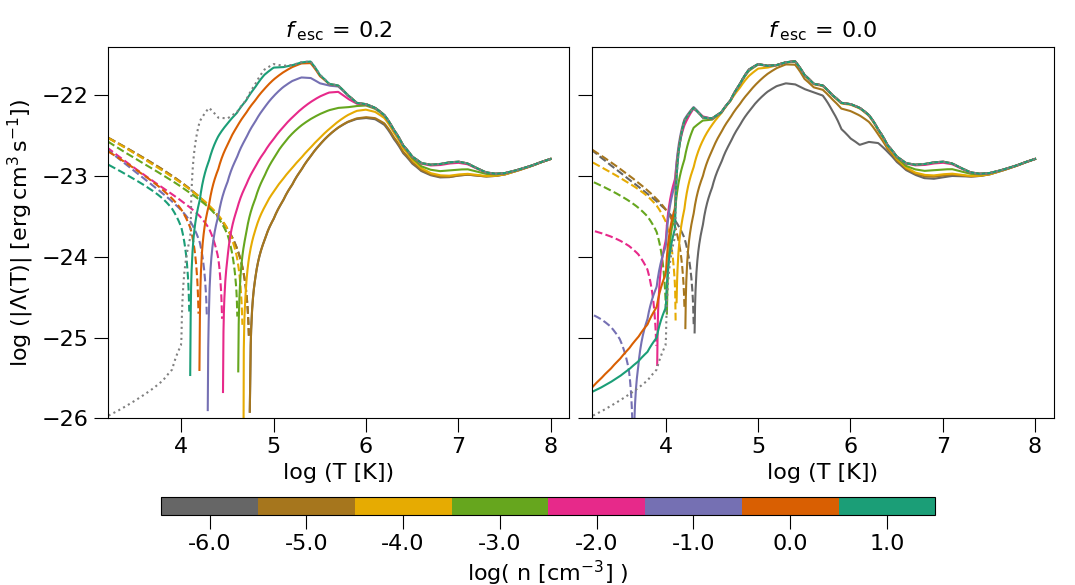
\includegraphics[width=1.0\textwidth]{plots/net_cooling.png}
    \caption{Net cooling function $\Lambda(n,T,r)$ as a function of the temperature $T$, for different values of the gas density $n$.
    %
    Note that the absolute value of $\Lambda$ is plotted: solid (dashed) lines represent positive (negative) values, i.e. net cooling (heating). 
    %
    The data for the cooling rates are taken from Gnedin \& Hollon \citep{gnedin2012cooling}, and we have used as input the values of the photoionization and photodissociation rates $\Gamma_{\mathrm{H}}$, $\Gamma_{\mathrm{He}}$, and $\Gamma_{\mathrm{LW}}$ derived in section  \ref{sec:radiation_fields}.
    %
    {\it Left}: case for $\fesc=0.2$, in which the ionizing radiation field is given by the sum of the flux from the galaxy ($\mathrm{SFR}=50\,\msun\mathrm{yr}^{-1}$) and the cosmic UVB at $z=6$. Results are shown at a galactocentric radius $r=1\,\mathrm{kpc}$. {\it Right}: case for $\fesc=0$. Ionizing radiation is only provided by the UVB. In both panels, The grey dotted line shows the cooling function under the hypothesis of Collisional Ionization Equilibrium (CIE; i.e., no radiation illuminating the gas).
    \label{fig:global_cooling}
    }
\end{figure*}

Having characterized the radiation fields that are present in the high-z galaxies' CGM, we can finally look at the thermal energy budget of the gas by focusing on the net cooling function $\Lambda(T)$. This is simply defined as the cooling function $\Lambda^\mathrm{(cool)}$ minus the heating function $\Lambda^\mathrm{(heat)}$, or, equivalently, as the total energy loss rate per unit volume ($\dot{\varepsilon}$) divided by the squared density ($\Lambda(T)=\dot{\varepsilon}/n^2$).

As already described, this function has a very complex dependence on many different physical variables, as all the atomic and molecular contributions to cooling and heating need to be taken into account. Even in the optically-thin case (and excluding the contribution of cosmic and X-rays), $\Lambda$ is a function of the temperature $T$, the gas density $n$, the fractional abundance $X_{ij}$ for the species $i$ (including atomic and ionic species, various molecules, and cosmic dust) at level $j$, and the mean specific intensity of the radiation field $J(\nu)$. 

A step forward in simplifying this function can be made by assuming that all the atoms and ions are in ionization equilibrium, i.e., the total (collisional + photoionization) rate of ionization is equal to the rate of recombination. Assuming that the levels are in equilibrium as well (excitation and de-excitation rates are identical), the net cooling function depends only on the gas temperature, density, and composition (metallicity), and, of course, on the radiation field strength $J(\nu)$. 

If no radiation is present, then equilibrium conditions are determined only by collisions: it is the so-called "\textit{Collisional Ionization Equilibrium}" (CIE) condition. Assuming CIE, we have seen that in the low-density limit the cooling rate (section \ref{sec:cooling}) does not depend on the density $n$, while the heating rate (sec. \ref{sec:heating}) is negligible as all the main heating processes rely on the energy carried by an incident radiation field. The only residual dependences, then, are temperature and metallicity; the grey dotted lines in figure \ref{fig:global_cooling} show the CIE cooling function for $Z=1\,Z_\odot$. 

As already mentioned, the presence of a UV radiation field acting on the gas affects the net cooling rate in two major ways: (a) it boosts the heating rate due to the photoelectric effect on gas and/or dust; (b) it alters the photoionization rates, reducing the abundances of cooling species such as \HI, \HeI, \CII and ultimately resulting in a lower emissivity of the gas. Overall, these effects tend to decrease significantly the value of $\Lambda$ at a given temperature, and they need to be carefully modeled to study the properties of the gas, especially in the low-density regime. 

In principle, the full spectral distribution of the specific intensity needs to be used in order to compute the abundance and the cooling/heating rates for every given species. However, this is very hard to do in practice, because it requires a lot of computational time. For this reason, in this work, we use the data tables created by Gnedin \& Hollon \citep{gnedin2012cooling} in order to determine the value of the net cooling function for the outflowing gas. 

The data tables are created by assuming low-density, optically thin gas in ionization equilibrium, and by neglecting the effects of cosmic and X-rays. Heating and cooling are computed using the \code{cloudy} spectral synthesis code \citep{ferland1994}, taking into input the temperature (T), density (n), and metallicity (Z) of the gas, as well as four other parameters that are meant to approximate well the complex dependence of $\Lambda$ on the incident radiation field. These parameters are: (1) the Lyman-Werner \HH photo-dissociation rate $\Gamma_\mathrm{H2}$; (2) the hydrogen photoionization rate $\Gamma_\mathrm{H}$; (3) the helium photoionization rate $\Gamma_\mathrm{He}$; (4) the \CVIion photoionization rate $\Gamma_\mathrm{CVI}$. They don't have any special meanings, but they are chosen because they can sample well the strength of the radiation field in all the regions of the spectrum, from the FUV one ($\Gamma_\mathrm{H2}$) to the EUV ranging from tens of eV ($\Gamma_\mathrm{H},\,\Gamma_\mathrm{He}$ to hundreds of eV ($\Gamma_\mathrm{CVI}$). 

We have already computed all these quantities for our physical environments in section \ref{sec:radiation_fields} (except for $\Gamma_\mathrm{CVI}$, which we set to a null value as it is important only for very hard radiation such as the one from quasars). Overall, three parameters determine the value of the total radiation fields (central galaxy + UVB): the galaxy's redshift ($z$), the star formation rate (SFR), and the escape fraction ($\fesc$); therefore, we can write the dependencies of the net cooling function as: $\Lambda = \Lambda(T,n,Z;r,\mathrm{SFR},z,\fesc)$. 

While the dependences on the SFR and on the redshift are sub-dominants, the escape fraction turns out to be a key factor governing the behaviour of the net cooling function. Given its uncertainty (section \ref{sec:first_lights_reionization}), we bracket all the possible values for the escape fraction by setting $\fesc = 0.2$ and $\fesc =0$. The former is consistent with the values used in most reionization studies \citep[e.g.,][]{Mitra15,Robertson15,Mitra18}, while the latter accounts for observations of very low $\fesc$ systems \citep[e.g.,][]{inoue2006escape,paardekooper2015first, ma2020no}. 

In figure \ref{fig:global_cooling}, we show the absolute value of the net cooling function, $|\Lambda(T)|$ for different values of the gas density (n), in the two extremal cases $\fesc=0.2$ (left panel) and $\fesc=0$ (right panel). The metallicity is taken to have a solar value ($Z=1\,Z_\odot$), while redshift and SFR are set to $z=6$ and $\mathrm{SFR}=50\,\msun\mathrm{yr}^{-1}$, respectively. For $\fesc=0.2$ the cooling function depends explicitly on the radius $r$: for displaying purposes, we fix $r=1\,\mathrm{kpc}$. In this case, as shown in section \ref{sec:radiation_fields}, the galaxy's radiation dominates over the UVB. For $\fesc=0$, instead, radiation from the galaxy is completely absorbed and the UVB is the only residual source of ionizing photons. 

Indeed, there are striking differences between the two $\fesc$ cases: in the left panel of figure \ref{fig:global_cooling} ($\fesc=0.2$), we see that the main effect of the strong galactic flux at a distance of $1$ kpc is to dramatically depress the ability of the gas to cool in the temperature range $10^{4-6}$ K, particularly for low gas densities. The decrease of the peaks is mostly produced by the fact that H (and partly also He) atoms, providing the main cooling channel via the excitation of the Ly$\alpha$ transition, become ionized and therefore unable to radiate efficiently. The equilibrium temperature, given by the condition $\Lambda=0$, is identified by the spikes in the curves, where a transition from cooling to heating-dominated regimes at lower $T$ takes place. The equilibrium values range in $\log T=4.1 - 4.7$, with the warmer solutions applying to lower densities. 

The situation is significantly different if ionizing radiation from the galaxy is not allowed to escape in the halo ($\fesc=0$, right panel). In this case, the much lower intensity of the UVB alone produces only a very limited suppression of the cooling function, and only for low densities, $n < 0.01\, \cc$. Equilibrium temperatures are consistently lower for $\fesc=0$, due to the smaller photoheating provided by the UVB. They range between $\log T=3.5 - 4.5$: this is consistent with the fact that the CGM/IGM of galaxies after reionization have temperatures around $10^4\,\mathrm{K}$, as they are not able to cool down any further due to the heating effect of the UVB. From this analysis, we conclude that the cooling function is heavily dependent on $\fesc$. As we will see, this has direct implications on the final emission of \CII in the model we are about to describe. 



 \section{Outflow model}\label{sec:outflow_model}



In this section, we can finally present our model in support of the \textit{outflow hypothesis} (sec. \ref{sec:theory_halos}). We focus on an instance of a normal star-forming, high-redshift galaxy, and we describe the properties of a galactic wind arising from the galaxy and expanding out into its CGM. Our aim is to derive physically-motivated density, velocity, and temperature radial profiles for the outflowing gas, and to use these quantities to compute the predicted \CII luminosity, in order to compare it with observations. 

We make use of the theoretical studies on SF-driven galactic outflows that we have introduced in section \ref{sec:model_outflows}. As a first exploratory investigation, we start by considering the CC85 model (sec. \ref{sec:cc85_model}). We summarize the crucial assumptions and results of the CC85 model in order to assess its validity and to look for possible improvements. The model considers the galaxy to be a sphere of radius $R$; hereafter, we take $R= 0.3\,\mathrm{kpc}$ as our fiducial value, as it is a good estimate for the average size of normal high-z galaxies \citep[e.g.,][]{Dayal:2018hft}. Energy and mass are injected inside the galaxy to model the effects of stationary SNe activity. The rates of energy ($\dot{E}$) and mass ($\dot{M}$) injection are:
\begin{subequations}
\begin{align}
    &\dot{E}=\alpha  E_{0,\mathrm{SN}} \nu_\mathrm{SN} \,\mathrm{SFR}\\
    & \dot{M}=\eta \, \mathrm{SFR},
\end{align}
\end{subequations}
where $E_{0,\mathrm{SN}} = 10^{51}\,\mathrm{erg}$ is the total energy released by a single SN, $\nu_\mathrm{SN}=10^{-2}\,\msun^{-1}$ is the rate of SNe per unit stellar mass, and SFR is the star formation rate. $\alpha$ and $\eta$ are the thermalization efficiency and the mass loading factor: these two parameters express the coupling between the wind and the ISM/SNe remnants in terms of energy and mass, respectively.
$\eta$ heavily affects the central gas density, and thus the general behavior of the system. Instead, the dependence of the physical variables on $\alpha$ is not as strong (especially considering radiative cooling effects, see e.g., eq. \ref{eq:eta_crit}), and to a first approximation, it can be fixed. For this reason, we have decided to set $\alpha=1$ (chosen accordingly to outflow observations by Strickland \& Heckman \citep{strickland2009supernova}), and retain $\eta$ as a free parameter. 

Eqs. \ref{eq:solinn} and \ref{eq:solout} express the solutions for the galactic wind arising in the CC85 setting for the inner and the outer regions, respectively. The solutions are expressed in terms of the Mach number $\mathcal{M}(r)=v(r)/c_s(r)$, where $c_s$ is the sound speed (eq. \ref{eq:sound_speed}), but can be recast in terms of physical quantities such as the velocity $v$, density $\rho$, and pressure $P$. A sketch for the radial profiles of these quantities can be found in figure \ref{fig:cc85} (note that in our discussion, we consider an adiabatic index $\gamma=5/3$). In figure \ref{fig:temp_CC85}, we show the same temperature profile for different values of the $\eta$ parameter, ranging from $0.2$ to $8.2$. We take a fiducial value for the star formation rate, $\mathrm{SFR}=50\,\msun\mathrm{yr}^{-1}$. For $r<R$ the temperature is roughly constant at $10^{7-8}\,\mathrm{K}$, with the exact value depending on $\eta$: more mass-loaded outflows are cooler. Beyond $R$, the temperature drops purely due to adiabatic cooling following the characteristic behavior $T\propto r^{-4/3}$. 

This drop in temperature is extremely important, as our goal is to create sufficient \CII emission in the gas, and this is possible only if the temperature gets lower than $T\lesssim10^4\,\mathrm{K}$. This is because carbon is collisionally ionized to \CIIIion (and higher ionization states) for temperatures above this threshold. Therefore, the presence of cool gas in the halo is essential to explain observations of \CII extended emission. Looking at figure \ref{fig:temp_CC85}, however, we realize that the adiabatic evolution assumed by the CC85 model results in a hot/warm outflow that has temperatures $T\gtrsim10^{4.5}\,\mathrm{K}$ (for all values of $\eta$) out to radial distances $r\gtrsim10\,\mathrm{kpc}$. Since the halos are observed in $10-15\,\mathrm{kpc}$ radii from the center, this implies that the CC85 model cannot account for the observed \CII emission. 

\subsection{Introducing cooling and gravity} \label{sec:cooling_gravity}



%

For this reason, motivated by the theoretical/observational studies of cool phases in outflows (section \ref{sec:outflows_cooling}), we abandon the adiabatic hypothesis by considering the possibility of gas heating and cooling. We have already described how a number of different works (in particular, Thompson et al. \citep{Thompson16}) have proved that, for high values of the mass loading factor $\eta$, energy losses are non-negligible in the CC85 model. We start from this point, and we aim at studying the transition between an adiabatic hot/warm mode in the outflow to a cool one due to the inclusion of radiative cooling.

We consider the same setting as the CC85 model: in particular, in the inner region ($r<R$), we retain the CC85's assumptions and thus recover the same solution eq. \ref{eq:solout} (for a discussion on this, see the end of section \ref{sec:outflows_cooling}). From this solution, we can express the physical conditions at the boundary region $r=R$ as (see also eqs. \ref{eq:bound_cc85_1}--\ref{eq:bound_cc85_3}):
\begin{subequations} \label{eq:boundary}
\begin{align}
&\rho(R)=\frac{\sqrt{2}}{4\pi}\,\frac{\dot{M}^{3/2}}{\dot{E}^{1/2}}\frac{1}{R^2}\propto {\rm SFR}\, \eta^{3/2}\\
&p(R)=\frac{3\sqrt{2}}{40\pi}\,\frac{\dot{M}^{1/2}\dot{E}^{1/2}}{R^2}\propto {\rm SFR} \,\eta^{1/2}\\
&v(R)=\frac{1}{\sqrt{2}}\,\frac{\dot{E}^{1/2}}{\dot{M}^{1/2}}\propto \eta^{-1/2}\,,\label{eq:v_boundary}
\end{align}
\end{subequations}
In the outer region, instead, we allow the gas to cool radiatively by introducing the net cooling function $\Lambda = \Lambda(T,n,Z;r,\mathrm{SFR},z,\fesc)$ in the hydrodynamical equations (eqs. \ref{eq:eul_cc85}). We obtain a new set of equations that can be integrated for $r>R$, using the physical relations at $r=R$ as boundary conditions for the system. 

\begin{figure}
	\centering
	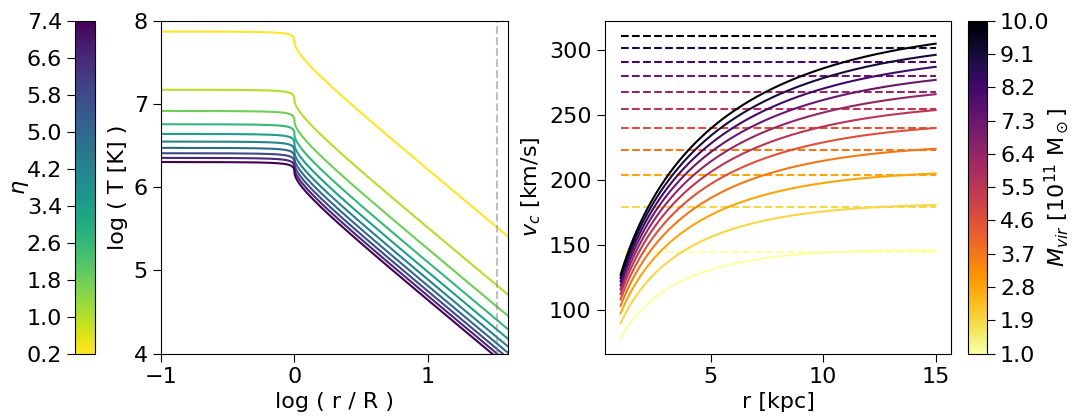
\includegraphics[width=1.0\textwidth]{plots/cc85+NFW.png}
	\caption{\textit{Left:} Outflow temperature (T) as a function of the radius (r) in the CC85 (adiabatic) model. The curves are calculated for $R=0.3\,\mathrm{kpc}$ and SFR$=50 \, \msun \rm yr^{-1}$. Different colors are used to map different values of the mass loading factor ($\eta$). \textit{Right}: local circular velocity as a function of the radius for a NFW \citep{NFW_profile} dark matter halo's density distribution. Different halos are color-coded according to their total virial mass. The dashed lines represent the maximum value reached by $v_c$, which is also the (constant) circular velocity profile it would result from an isothermal sphere distribution.
	\label{fig:temp_CC85}
	}
\end{figure}

However, we have yet to take another step forward. Since the outflow is slowed down because of energy losses, neglecting the dark matter halo's gravitational influence is not possible anymore. For this reason, we include a gravitational potential $\varphi(r)$ created by a dark matter distribution $\rho(r)$ in the Euler equation (eq. \ref{eq:eul2_cc85}). Exploiting the assumption spherical symmetry, as well as the Gauss theorem, we can write the radial gradient of the potential as:
\begin{align}
\frac{\d \varphi(r)}{\d r}=\frac{G M(r)}{r^2} = \frac{v_c^2(r)}{r}
\end{align}
In this expression, $M(r)$ is the total mass contained in a sphere of radius $r$, and $v_c(r)$ is the local circular velocity:
\begin{align}
v_{c}(r) &= \sqrt{\frac{GM(r)}{r}}
\label{eq:v_c_definition_model}
\end{align}
In principle, one should also include the gravitational contribution due to the baryonic component in the galaxy disk. However, we neglect this term, as the disk potential decreases faster than the DM halo potential as the galactocentric distance increases. This implies that beyond a kpc scale (where the physics of the outflow becomes more interesting) the disk contribution tends to be irrelevant, and dark matter dominates the gravitational energy budget.

As described in section \ref{sec:halos}, two main choices are possible for the dark matter halo's density profile. A simpler solution can be obtained by taking an isothermal sphere profile (eq. \ref{eq:iso_sphere}): in this case, $M(r)\propto r$, and then $v_c(r) = {\rm const}$. Therefore, with this choice, gravity can be implemented in a fairly straightforward way. However, such a profile builds up a lot of mass in the halo's core, resulting in a very strong slowing effect on the outflow, especially in the region where the outflow velocity is still relatively small. 

This motivates us to search for a different, more promising solution. With this respect, a more physically motivated candidate is the Navarro-Frenk-White (NFW) profile (eq. \ref{eq:nfw_profile}). This profile has a flatter core, and it mimics the observed/simulated profiles much more faithfully (sec. \ref{sec:halos}). The radial dependence of $v_c(r)$ -- or, equivalently, $M(r)$ -- is not as simple, but it still can be obtained analytically by integrating the density profile $\rho(r)$ in a volume of radius $r$:
\begin{align}
M(r) = \frac{M_{vir}}{A_\mathrm{NFW}}\, \left(\log\left(\frac{r_s + r}{r_s}\right) + \frac{r_s}{r_s + r} -1\right) 
\end{align}
where $M_{vir}$ is the virial mass of the halo, $A_\mathrm{NFW} = \log(1+c_N) - c_N/(1+c_N)$, and $r_s$ is the halo "scale radius", which is related to the virial radius via the \textit{concentration parameter} $c_N = r_{vir}/r_s$. Obviously, this formula holds valid only for $r<r_{vir}$. The virial radius can be determined from the virial mass by fixing a conventional overdensity $\delta_c = 200$, and knowing the average density ($\Bar{\rho}(z)$) of the universe at redshift $z$:
\begin{align}
r_{vir} = \left(\frac{3M_{vir}}{\Bar{\rho}(z)\,4\pi \delta_c}\right)^{1/3}
\end{align}
We obtain the concentration parameter (at a given virial mass and a given redshift) from the fit realized by Dutton \& Macciò \citep{dutton2014cold}. $M_{vir}$ and $z$ are therefore the only free parameters that need to be fixed in order to characterize completely the halo's gravitational potential $\varphi(r)$. For our convenience, we replace $M_{vir}$ with an equivalent parametrization, by introducing the global circular velocity $v_c = \sqrt{GM_{vir}/r_{vir}}$. 

Figure \ref{fig:temp_CC85} shows the radial NFW profiles for the local circular velocity $v_c(r)$, for different choices of the virial mass $M_{vir}$ -- or, equivalently, of the global circular velocity $v_c$. Note that, in the case of an isothermal sphere, the global and the local circular velocity are the same everywhere. Since $v_c$ is also the maximum value assumed by the local circular velocity $v(r)$, this implies that the effects of an isothermal sphere are much more dramatic than the ones of an NFW profile. Hereafter, we will consider the NFW prescription as the fiducial choice in our model.



\subsection{Physical profiles for the outflow} \label{sec:outflow_profiles}

Having specified the conditions for cooling and gravity, we can finally rewrite the hydrodynamical equations for the outflow in the region $r>R$: these are mass conservation, Euler equation, and energy conservation (eqs. \ref{eq:eul1_cc85}--\ref{eq:eul3_cc85} with $q=Q=0$). Euler equation changes because of the presence of a gravitational force due to the dark matter halo's potential. The energy conservation equation, on the other hand, needs to take into account the energy losses due to radiative cooling. It is convenient to write the energy balance making use of the first principle of thermodynamics:
\begin{align}
-\d \varepsilon = \d u - \frac{P}{n}\,\d n,
\end{align}
where $\d \varepsilon$ is the total energy lost (note the minus sign) by the system, and $\d u$ is the change in the internal energy; both quantities are defined per unit volume. Exploiting this relation, we can write the energy balance for the spherical flow as:
\begin{align}
-\dot{\varepsilon}  = uv \,\frac{1}{T}\frac{\d T}{\d r} - Pv\,\frac{1}{n}\frac{\d n}{\d r} = - n^2 \,\Lambda,
\end{align}
where we have used the definition of the net cooling function $\Lambda = \Lambda^\mathrm{(cool)}-\Lambda^\mathrm{(heat)}$. 

Given these premises, we can write the set of equations describing the outflow as: 
\begin{subequations}
\begin{align}
&\frac{1}{r^2}\der{}{r}(r^2v\rho) =0, \label{eq:neweul1}\\
&\rho v\der{v}{r} = -\der{p}{r} - \rho \der{\varphi}{r} \label{eq:neweul2}\\
&\left(\frac{1}{T}\der{T}{r} - (\gamma-1)\frac{1}{\rho}\der{\rho}{r}\right) v k_B T = - (\gamma-1) n \Lambda \label{eq:neweul3}
\end{align}
\end{subequations}
Combining these three equations we get a first order system of ODE that can be integrated numerically to solve for the variables $\rho$, $v$, and $T$. It is convenient to express these equations in terms of the flow Mach number $\mathcal{M}=v/c_s$, the gravitational Mach number $\mathcal{M}_g=v_c/c_s$, and the cooling time $\tau_\Lambda =  k_B T/n\Lambda$ (eq. \ref{eq:tcool}):
\begin{subequations}
\begin{align}
&\der{\log\rho}{\log r}=2 \left(\frac{\mathcal{M}^2-\mathcal{M}_g^2/2}{1-\mathcal{M}^2}\right)- \frac{r}{\lambda_\Lambda}\left(\frac{1}{1-\mathcal{M}^2}\right) \label{eq:cooling_model_equations_n}\\
&\der{\log v}{\log r}=\left(\frac{\mathcal{M}_g^2-2}{1-\mathcal{M}^2}\right)+\frac{r}{\lambda_\Lambda}\left(\frac{1}{1-\mathcal{M}^2}\right) \label{eq:cooling_model_equations_v}\\
&\der{\log T}{\log r}={2(\gamma-1)}\left(\frac{\mathcal{M}^2-\mathcal{M}_g^2/2}{1-\mathcal{M}^2}\right)-\frac{r}{\lambda_\Lambda}\left(\frac{1-\gamma\mathcal{M}^2}{1-\mathcal{M}^2}\right)\,, \label{eq:cooling_model_equations_T}
\end{align}
\label{eq:cooling_model_equations}
\end{subequations}
where $\lambda_\Lambda=(\gamma/(\gamma-1)) v \tau$ is the cooling length.

The cooling function $\Lambda$ (and, in turn, the cooling length $\lambda_\Lambda$) depends on a number of parameters that needs to be fixed to solve the system of equations for the outflow: the metallicity ($Z$), the redshift ($z$), the star formation rate (SFR), and the escape fraction ($\fesc$). The gravitational potential adds a further dependence on the global circular velocity ($v_c$) of the halo. In what follows, we set some values for these parameters, in order to solve the equations in some cases of interest and discuss the resulting solutions for the outflows. We will investigate further other choices for the parameters in section \ref{sec:CII_emission}. 

First of all, we consider solar metallicity for the outflow ($Z=1\,Z_\odot$); this is equivalent to say that the ISM of high redshift galaxies has metallicities equal to (or close to) solar values. This statement is supported by simulations of high-z galaxies \citep[e.g.,][]{pallottini2017} and by the extrapolation of the local mass-metallicity relation to higher redshifts \citep[e.g.,][]{mannucci:2012}. Redshift, star formation rate, and circular velocity can be gauged with sufficient accuracy from observations. For this reason, we will set their values guided by observations in the next chapter. Here, we employ some fiducial values that are reasonable for normal, star-forming, high-z galaxies: $z=6$, $\mathrm{SFR}=50\,\msun\mathrm{yr}^{-1}$, $v_c = 200\,\kms$. Since $\fesc$ can change dramatically the energy balance of the gas, we study here the same two configurations $\fesc=0.2$ and $\fesc =0$ that we have considered in section \ref{sec:cooling_function}.


Figure \ref{fig:global_profiles} shows the radial profiles of the key hydrodynamical variables, $v, n, T$ for different values of the mass load parameter, $\eta$. In the left panel, we set $\fesc=0.2$, while in the right panel consider only the UVB radiation by setting $\fesc=0$. The first thing to note is that both velocity and density are not strongly affected by the choice of different values for the escape fraction $\fesc$. Therefore, we can conclude that a different prescription for the radiation impinging on the gas has only a secondary effect on its density and velocity. 

In both columns, for low values of $\eta$ ($\eta \lesssim 1$), the radial asymptotic dependencies are the same as the CC85 model: $v \approx \mathrm{const.}$ and $n\propto r^{-2}$. This implies that cooling, for these low-$\eta$ values, is not efficient enough, and thus the evolution is approximately adiabatic in the whole range of radii considered. This is supported by the temperature profiles of these outflow modes -- which resembles a power-law in all $\fesc$ scenarios -- and it is perfectly in line with the analytical estimates we have outlined in section \ref{sec:outflows_cooling}. 

When $\eta$ increases to values higher than unity, instead, cooling starts to become efficient, and the evolution changes considerably. The initial density becomes high enough for gravity to become important. This reduces the velocity up to a stalling radius, $r_{\rm stop}$, where the velocity drops to zero. The position of the stalling point moves closer to the galaxy as $\eta$ increases. Because of the gas slowing down, the density tends to increase in the outer regions of the outflow, becoming greater and greater as the distance approaches the stalling radius $r_\mathrm{stop}$. 

We note that the presence of a stalling radius is a consequence of our assumptions of stationarity and spherical symmetry. In a time-dependent scenario, the gas, after being halted by the gravitational potential of the halo, would fall back forming a galactic fountain and mixing with the outflow. Our semi-analytic study cannot capture the complexity of this process. However, we believe that studying for which conditions gravity can halt the gas and thus increase its density in the outer layers of the outflow is already an important step towards a full comprehension of this complex phenomenon.

Cooling introduces new, striking features in the temperature profiles shown in the lower panels of figure \ref{fig:global_profiles}. For high values of the mass loading factor ($\eta \gtrsim 1$) the gas starts cooling at a distance $r_{\mathrm{cool}}$ that gets smaller as $\eta$ increases. The cooling is quite rapid, supporting the "catastrophic cooling" scenario already studied by several previous works (see section \ref{sec:outflows_cooling}). After cooling has taken place, the gas temperature evolution depends on our choice for $\fesc$. If we include the radiation from the galaxy (i.e., $\fesc=0.2$), cooling stops at an equilibrium temperature of around $10^4 \,\mathrm{K}$. Beyond the cooling radius, the outflow is subject to a quasi-isothermal expansion. For $\fesc=0$, the temperature profiles are quite different, as expected from the different behaviors of the cooling function (figure \ref{fig:global_cooling}). The gas is able to cool down further to a temperature of a few hundred degrees. At larger radii, however, the gas slowly heats up, as the net cooling function takes negative values (i.e. the photoionization heating takes over as density decreases). As we will show in the next few paragraphs, temperatures of a few $\times 100$K allow a significant presence of \CIIion, and thus a potentially observable \CII emission. 




\begin{figure*}
    \centering
    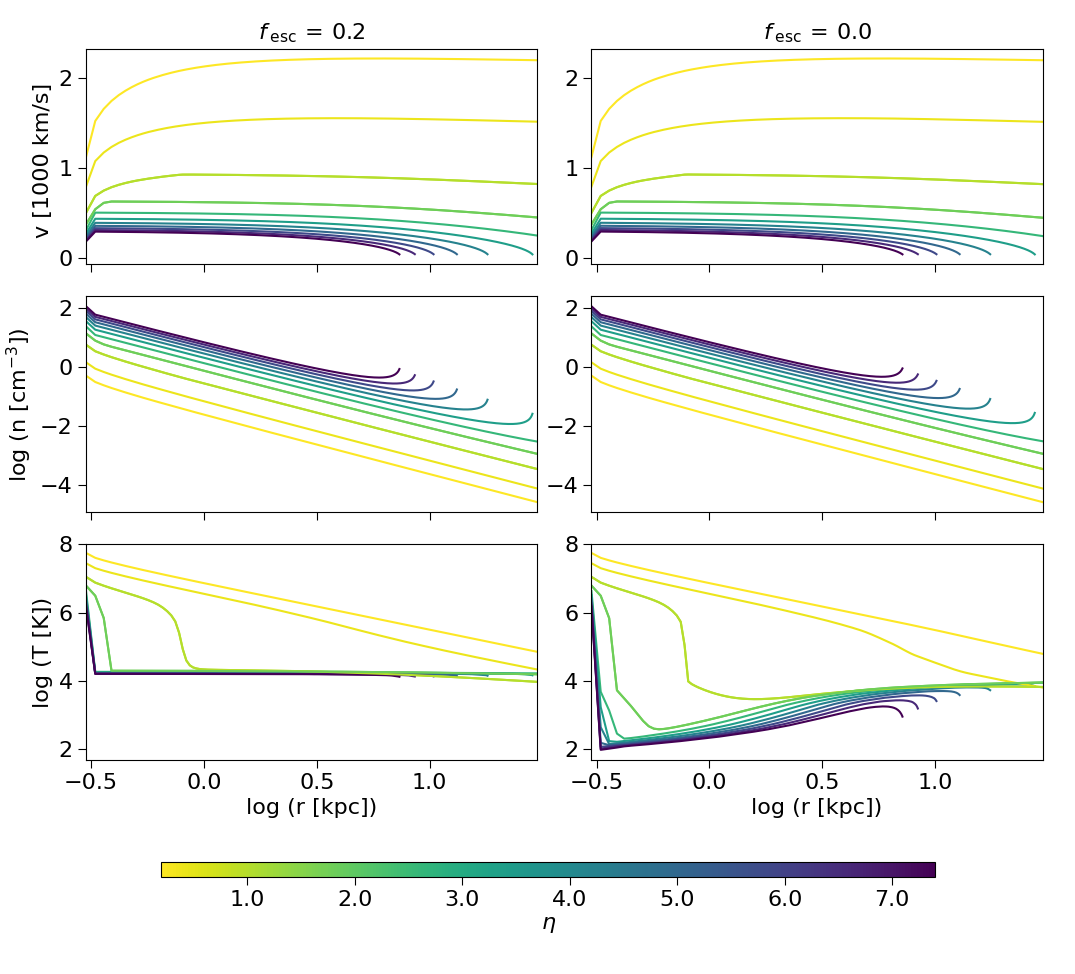
\includegraphics[width=1.\textwidth]{plots/profiles.png}
    \caption{Radial profiles of key outflow thermodynamical variables obtained for our model including cooling and gravity (eqs. \ref{eq:cooling_model_equations}). Shown are the two cases $\fesc=0.2$ (left column), and $\fesc=0$ (right).
    \textit{Top row}: Velocity ($v$). For high values of the mass loading factor $\eta$, gravity slows down the outflow until a stalling radius at which $v=0$ is reached.
    %
    \textit{Middle}: Density ($n$). The radial dependence of the density is generally $n\propto r^{-2}$, but its value increases as the gas slows down due to gravity.
    %
    \textit{Bottom}: Temperature ($T$). Note the different temperature profiles beyond the cooling radius. For $\fesc=0$ the outflow cools to lower temperatures and reaches the equilibrium value of $T\approx10^4\,\mathrm{K}$ only at much larger radii.  
    \label{fig:global_profiles}
    }
\end{figure*}

\begin{comment}

\subsection{Some analytical considerations} \label{sec:analytical}

WRITE ABOUT ANALYTICAL APPROACH ETC

MENTION THE SHARP DEPENDENCE OF V ON ETA

The dependence of the stalling radius, $r_\mathrm{stop}$, on the SFR can be inferred from eq. \ref{eq:cooling_model_equations_v}. For temperatures $T\approx10^{2-4}\, \mathrm{K}$, the flow is highly supersonic. Also, the cooling length of the gas remains larger than the outflow extent. Hence, using these approximations it is straightforward to obtain an analytical solution for the profile $v(r)$ (see also \citet{Thompson16}), from which it follows that
\begin{align}
r_\mathrm{stop} \approx r_\mathrm{cool}\,e^{v^2(r_\mathrm{cool})/2v_c^2},
\end{align}
which implies that $r_\mathrm{stop}$ increases with the cooling radius, $r_\mathrm{cool}$. As the latter has a strong inverse dependence on the outflow rate $\eta {\rm SFR}$ \citep{Thompson16}, a higher SFR value results in a smaller $r_\mathrm{stop}$. Hence, beyond $r_\mathrm{stop}$ the emission drops to zero. 
%
\end{comment}

\subsection{Ionization state of the gas}\label{sec:ionization_structure}


Knowing the density and temperature of the outflowing gas, we can compute the ionization state of different species as a function of the radial distance from the galaxy. This is an important step towards the computation of the final \CII emission, as the energy emitted by the \CII transition depends on the numerical abundances of free electrons and singly ionized carbon (eq. \ref{eq:CII_cooling}).

We start by assuming that the free electron density is equal to the \HI density, i.e., $n_e \approx n_p$. This means that we neglect contributions from other ionized species, such as He and C, because of their lower abundance and/or higher (for He) ionization potential. Then, assuming ionization equilibrium, we write the statistical balance for hydrogen ionization by equating the rates of photoionization ($\Gamma_{\mathrm{H}}$) and collisional ionization ($k_{\mathrm{H}}$) with the recombination rate ($\eta_{\mathrm{H}}$):
\begin{align}
n_\mathrm{H} \Gamma_{\mathrm{H}} + n_\mathrm{H} n_e k_{\mathrm{H}} = n_e\, n_{p} \,\eta_{\mathrm{H}}
\label{eq:ion_bal}
\end{align}
We have already computed the value of $\Gamma_\mathrm{H}$ in section \ref{sec:radiation_fields}. For $\eta_H$, we use the power-law approximation to Case B radiative recombination given by \citet{tielens2005book},
\begin{align}
\eta_\mathrm{H} = 4.18 \times 10^{-13} \, \bigg(\frac{T}{10^4 \, \mathrm{K}}\bigg)^{-0.75} \,\, \mathrm{cm}^3\, \mathrm{s}^{-1}
\label{eq:beta_H}
\end{align}
$k_\mathrm{H}$ is taken from \citet[][Appendix B]{bovino:2016aa}.

Using $n_\mathrm{p} + n_\mathrm{H} = \mathcal{A}_\mathrm{H} n$, where $A_\mathrm{H}$ is the cosmic hydrogen abundance ($A_{\mathrm{H}} = 0.76$ for solar composition \citep{asplund2009}), $n$ is the total gas density, and defining $x_\mathrm{e}=n_\mathrm{e}/n$, we can recast eq. \ref{eq:ion_bal} in the following form:
\begin{align}
(\eta_\mathrm{H}+k_\mathrm{H})\,x_e^2 + \bigg(\frac{\Gamma_{\mathrm{H}}}{\mathcal{A}_H n}-k_\mathrm{H}\bigg)\,x_e - \frac{\Gamma_\mathrm{H}}{\mathcal{A}_H n}= 0
\label{eq:ne}
\end{align}
Solving this quadratic equation, the H ionization fraction $x_e$ can be obtained. 
 
We now turn to carbon, and write the equivalent ionization equations assuming a detailed balance among three states of C atoms ionization: neutral (with number density $n_{\mathrm{CI}}$), singly ionized ($n_{\mathrm{CII}}$), and doubly ionized ($n_{\mathrm{CIII}}$).
\begin{subequations}
\begin{align}
n_\mathrm{CI} \Gamma_{\mathrm{CI}} + n_\mathrm{CI} n_e k_{\mathrm{CI}} &=n_e\, n_\mathrm{CII} \,\eta_{\mathrm{CII}}\\
n_\mathrm{CII} \Gamma_{\mathrm{CII}} + n_\mathrm{CII} n_e k_{\mathrm{CII}}&=n_e\, n_\mathrm{CIII} \,\eta_{\mathrm{CIII}}
\end{align}
\end{subequations}
The photoionization, collisional ionization, and recombination coefficients are $\Gamma_{\mathrm{CI}}$, $\Gamma_{\mathrm{CII}}$, $k_\mathrm{CI}$, $k_\mathrm{CII}$, and $\eta_{\mathrm{CII}}$, $\eta_{\mathrm{CIII}}$, respectively. Again, we can write the constraint $n_\mathrm{CI}+n_\mathrm{CII}+n_\mathrm{CIII}=\mathcal{A}_\mathrm{C} n \equiv n_\mathrm{C}$, with the carbon abundance taken to be equal to the Solar value $\mathrm{A}_{\mathrm{C}} = 2.69 \times 10^{-4}$ \citep{asplund2009}. Using this relation, we can solve the equations above and obtain the ionization fraction of carbon $x_\mathrm{CII}= n_\mathrm{CII}/n_\mathrm{C})$:
\begin{align}
x_\mathrm{CII} = \bigg(1+\frac{\Gamma_{\mathrm{CII}}}{n_e\,\eta_{\mathrm{CIII}}}+\frac{n_e\,\eta_{\mathrm{CII}}}{\Gamma_{\mathrm{CI}}+n_e k_\mathrm{CI}}+ \frac{k_\mathrm{CII}}{\eta_\mathrm{CIII}}\bigg)^{-1} \label{eq:densityCII}
\end{align}

The photoionization rates $\Gamma_{\mathrm{CI}}$ and $\Gamma_{\mathrm{CII}}$ have also been computed in section \ref{sec:radiation_fields} (eqs. \ref{eq:ionization_states_gal}--\ref{eq:ionization_states_uvb}) taking into account both the galaxy and the UVB contributions. Recombination rates must include both radiative and dielectronic recombination. For these, we use the following approximations \citep{tielens2005book}: 
\begin{subequations}
\begin{align}
\eta_\mathrm{CII} &= 10^{-13} \bigg[ 4.66 \bigg(\frac{T}{10^4 \, \mathrm{K}}\bigg)^{-0.62} + 1.84  \bigg]\,\, \mathrm{cm}^3\, \mathrm{s}^{-1}\\
\eta_\mathrm{CIII} &=10^{-12} \bigg[ 2.45  \, \bigg(\frac{T}{10^4 \, \mathrm{K}}\bigg)^{-0.65} + 6.06 \bigg]\,\, \mathrm{cm}^3\, \mathrm{s}^{-1}
\end{align}
\end{subequations}
%
Finally, we take the collisional ionization rates, $k_\mathrm{CI}$ and $k_\mathrm{CII}$, from \citet[][Table 1]{voronov_practical_1997}.


The resulting ionization radial profiles are shown in figure \ref{fig:global_ionization}. Again, there are dramatic differences between the two cases $\fesc=0.2$ and $\fesc=0$. If $\fesc=0.2$, the ionization radiation coming from the galaxy has dramatic effects on the gas: both H and C atoms are strongly photoionized by this radiation, and they are largely found in the form of \HII and \CIIIion. In particular, the fraction of singly ionized carbon is $x_{\rm CII}=n_{\rm CII}/n_C \lesssim 10^{-3}$. Such a small abundance of \CIIIion is problematic, because it suppresses the \CII emission and thus it is not compatible with the observations of \CII halos that we aim to explain. 

The $\fesc=0$ case, on the other hand, gives results that are much more promising. In the right panels of figure \ref{fig:global_ionization}, we see that models that undergo catastrophic cooling can produce considerable amounts of \CIIion. As the gas cools to a few hundred degrees K beyond $r_{\rm cool}$, carbon recombines, and $x_{\rm CII} \gsim 0.5$ in most cases but the lowest values of $\eta$. The outflow is essentially neutral as H has also largely recombined. As the outflow temperature increases again towards larger radii, because of the UVB photoheating, \CIIion ions are collisionally (and photo-) ionized, and their abundance decreases, albeit remaining significant. 

Therefore, our model seems to hint at the fact that only very low values of the escape fraction $\fesc$ are compatible with an appreciable presence of \CII in the outflow. This implies that the outflow hypothesis may be compatible with observations only if dust and/or \HI absorption prevents the galaxy's radiation from ionizing the \CIIion in the wind. For this reason, in the following analysis, we will concentrate on the case $\fesc=0$, which is the only one to be compatible with observations. The behavior of the gas ionization state in the outflow raises the interesting possibility that outflows might be used to indirectly probe the escape fraction $\fesc$. We will return to this point later on.


\begin{figure*}[t]
    \centering
    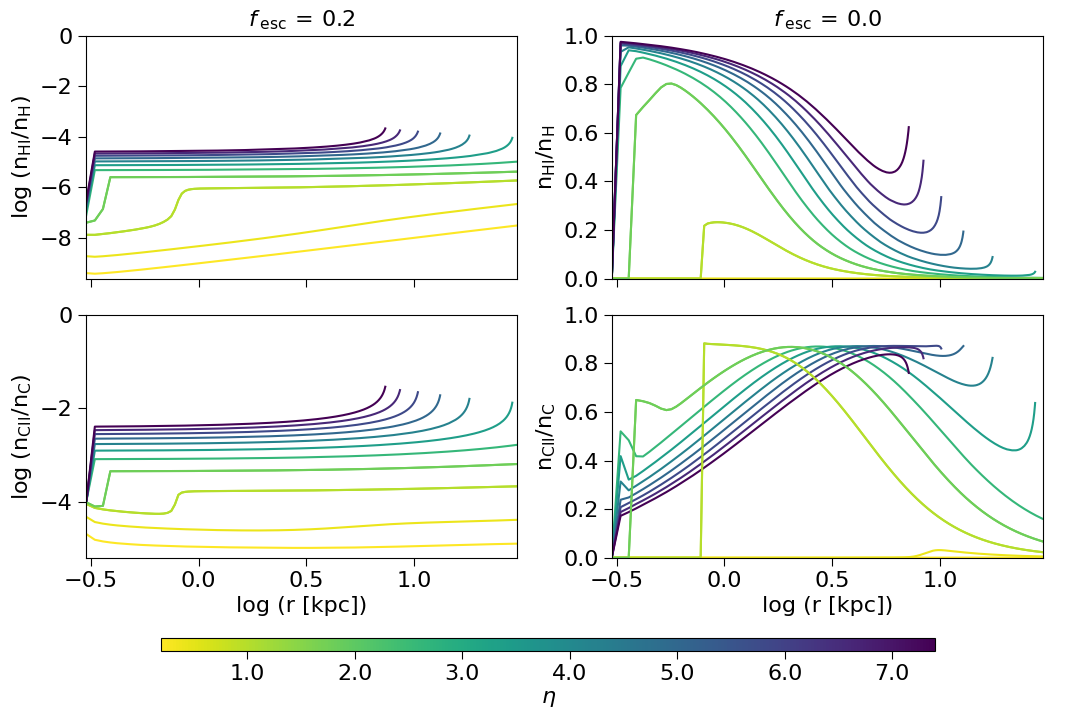
\includegraphics[width=1.0\textwidth]{plots/ions.png}
    \caption{Outflow radial ionization profiles. Shown are the two cases $\fesc=0.2$ (left column), and $\fesc=0$ (right). Note the linear scale in the right panels.
    %
    \textit{Top row}: Neutral hydrogen fraction (eq. \ref{eq:ne}). \textit{Bottom}: Singly ionized carbon fraction from eq. \ref{eq:densityCII}.
    \label{fig:global_ionization}
    %
    }
\end{figure*}


\section{[CII] line emission}\label{sec:CII_emission}


The emissivity of the \CII line $\dot{\varepsilon}_\mathrm{CII} = n^2 \Lambda^\mathrm{(cool)}_\mathrm{CII}$ can simply be determined using eq. \ref{eq:CII_cooling}. It is a function of the gas temperature $T$, of the free electron density $n_e$, and of the \CIIion density $n_\mathrm{CII}$. Using the ionization fractions computed at the end of last section, these densities can be expressed as a function of the gas density $n$:
\begin{subequations}
\begin{align}
&n_e = x_e(r)\,\mathcal{A}_\mathrm{H}\,n(r)
&n_\mathrm{CII} = x_\mathrm{CII}(r)\,\mathcal{A}_\mathrm{C}\,n(r)
\end{align}
\end{subequations}
Then, the final expression for the emissivity as a function of the radius $r$ is:
\begin{align}
 \dot{\varepsilon}_\mathrm{CII} (r) = 8.2\times10^{-21} \,\left(\frac{92\,\mathrm{K}}{T(r)}\right)^{1/2}\,n^2(r)\,\mathcal{A}_\mathrm{H}\,\mathcal{A}_\mathrm{C}\,x_e(r) \,x_\mathrm{CII}(r) \,e^{-92\ \mathrm{K}/kT(r)}\,\,\mathrm{erg}\,\mathrm{s}^{-1}\mathrm{cm}^{-3} \label{eq:emissivity_CII}
\end{align}
From the emissivity, the \CII surface density ($\Sigma_\mathrm{CII}$) can be obtained. The computation of $\Sigma_\mathrm{CII}$ is simplified by noting that, in most cases, the \CII emission is optically thin \citep[e.g.,][]{osterbrock1992}. Then, the \CII surface density at a point $(x,y)$ in the image plane is simply obtained by integrating the emissivity along the line of sight (parametrized by $h$:
\begin{align}
\Sigma_\mathrm{CII}(x,y)=\int\dot{\varepsilon}_\mathrm{CII}(s)\,\d s
\label{eq:emissivity}
\end{align}
Exploiting the symmetry of our model, we can express $\Sigma_\mathrm{CII}$ as a function of a single variable, the impact parameter $b$ (i.e., the distance between the line of sight and the center of the galaxy). Eq. \ref{eq:emissivity} can then be written as:
\begin{align}
\Sigma_\mathrm{CII}(b)&=\int_{-\infty}^{+\infty} \dot{\varepsilon}_\mathrm{CII}(r(s))\, \d s = 2 \int_{b}^{+\infty} \dot{\varepsilon}_\mathrm{CII}(r)\, \frac{r}{\sqrt{r^2 - b^2}}\,\d r \,
\label{eq:final_intensity}
\end{align}
Obviously, this final \CII surface density depends implicitly on a much greater number of parameters, such as mass loading factor, metallicity, redshift, SFR, circular velocity, and escape fraction. This dependence is hidden inside the thermodynamical variables and the ionization states in the outflow.  If all these parameters are set, then we have a prescription to compute the expected \CII emission, and we can compare this quantity with observations. However, in this discussion, we have neglected an important effect that may have a relevant effect on our final \CII emission. This effect is caused by the interaction of CMB photons with \CIIion atoms, and it is the subject of the next paragraph. 

\subsection{Correcting for the CMB suppression}\label{sec:CMB_suppression}


\begin{figure*}
    \centering
    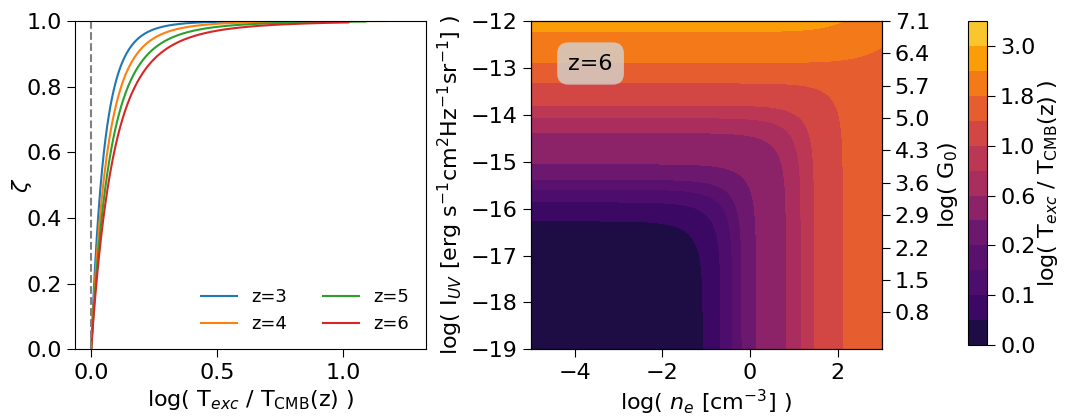
\includegraphics[width=1.\textwidth]{plots/cmb_theory.png}


    \caption{\textit{Left}: CMB suppression factor $\zeta$ (eq. \ref{eq:suppression_factor}) as a function of the ratio between $T_\mathrm{exc}$ and $T_\mathrm{CMB}(z)$, for different values of the redshift $z$. \textit{Right}: color map showing the ratio between the excitation temperature and the CMB one ($T_\mathrm{exc}/T_\mathrm{CMB}(z)$), computed at redshift $z=6$, as a function of the free electrons density $n_e$ and the UV intensity $I_{UV}$ at $1330$ \AA.
    \label{fig:cmb_intro}
    }
\end{figure*}


At high redshifts, new physical mechanisms become important, and they have to be taken into account by theoretical models. The CMB suppression is an instance of these effects that characterize the high redshift universe. As we have described in section \ref{sec:intro_cosmo}, the Cosmic Microwave Background is relic radiation that pervades the whole universe from the time of last-scattering. CMB photons follow a black body distribution  (eq. \ref{eq:black_body}) with an average temperature that scales with redshift as $T_\mathrm{CMB}(z) = T^{(0)}_\mathrm{CMB} (1+z)$ ($T^{(0)}_\mathrm{CMB}=2.73\,\mathrm{K}$ is the temperature of the CMB we measure today). Therefore, as redshift increases, CMB photons are more energetic, and they start to have a non-negligible effect on atomic transitions, particularly in the FIR/radio region of the spectrum. 

This effect is twofold: on one side, the presence of pervading radiation acting on the gas affects the level populations, and hence the \CII transition rate; on the other, any \CII emissions will be observed against a uniform CMB background, and this needs to be taken into account when computing the \CII surface density. 

The CMB radiation alters the level balance equation (eq. \ref{eq:level_eq}) by providing an absorption and a stimulated emission rates:
\begin{equation}
    n_l \,n_e\,\gamma_{lu} + n_l \,B_{lu}\, I(\nu_*) = n_u\,n_e\,\gamma_{ul} + n_u\,A_{ul} + n_u\, B_{ul} \,I(\nu_*)
\end{equation}
In this equation, we are considering the two-level system created by the \CIIion fine structure doublet, $^2P_{3/2}-\,^2P_{1/2}$; the transition associated with this system has a frequency $\nu_* = 1900\,\mathrm{GHz}$. $n_l$ and $n_u$ are the numeric densities of the two levels, and $n_e$ is the density of free electrons (the main collisional partners for \CII, see sec. \ref{sec:cooling}). $I(\nu) = B(\nu, z)$ is the (black-body) specific intensity of the CMB radiation. The Einstein coefficients and collisional rates have already been defined in section \ref{sec:cooling} and can be found in \citet{gong2012}. This balance equation is correct for a pure two-level system. However, \CII contains many other levels, and transition with more energetic levels is possible if the radiation illuminating the gas is energetic enough. In particular, in the presence of FUV radiation at $1330$ \AA, electrons can be pumped from the $^2P_{3/2}$ ($^2P_{1/2}$) level to $^2D_{3/2}$ at $1335.66$ \AA ($1334.53$ \AA). Then, this pumping effect can lead to the CII fine structure transitions $^2D_{3/2}\rightarrow \,^2 P_{3/2} \rightarrow \,^2 P_{1/2}$, resulting in a mixing of the levels we are interested in. Since we are including FUV radiation from the UV background and the parent galaxy, we need to include the UV excitation and de-excitation rates in the balance equation, to account for this \textit{UV-pumping} effect \citep[for more details, see][]{gong2012, vallini2015, kohandel:2019}. These rates are given by the following expressions \citep{field}:
\begin{align}
    P_{ul}^\mathrm{(UV)} &= \frac{g_k}{g_u}\frac{A_{kl}A_{ku}}{A_{kl}+A_{ku}}\left(\frac{c^2 I_\mathrm{UV}(\nu_{ku})}{2h\nu_{ku}^3}\right)&
    P_{lu}^\mathrm{(UV)} &= \frac{g_k}{g_l}\frac{A_{kl}A_{ku}}{A_{kl}+A_{ku}}\left(\frac{c^2 I\mathrm{UV}(\nu_{kl})}{2h\nu_{kl}^3}\right)
\end{align}
where “$k$” stands for the level $^2D_{3/2}$ ($g_k = 4$ is the level degeneracy), and $I_\mathrm{UV}$ is the UV radiation intensity. $A_{kl} = 2.41\times10^8\,\mathrm{s}^{-1}$ ($\nu_{kl}$) and $A_{ku} = 4.76\times 10^7\,\mathrm{s}^{-1}$ ($\nu_{ku}$) are the Einstein
coefficients (frequencies) of the $^2D_{3/2}\rightarrow \,^2P_{1/2}$ and $^2D_{3/2} \rightarrow \,^2P_{3/2}$ transitions, respectively.  

Accounting for the UV-pumping effect, yields:
\begin{equation}
    n_l \,n_e\,\gamma_{lu} + n_l \,B_{lu}\, I(\nu) + P_{lu}^\mathrm{(UV)} = n_u\,n_e\,\gamma_{ul} + n_u\,A_{ul} + n_u\, B_{ul} \,I(\nu) + P_{ul}^\mathrm{(UV)}
\end{equation}
This equation can be rewritten by introducing the excitation temperature $T_\mathrm{exc}$, in the same exact way as eq. \ref{eq:t_exc}. Using the relations linking the three Einstein coefficients (eqs. \ref{eq:einstein_coeff}), and the two collisional rates (eq. \ref{eq:coll_rates}), we obtain the following expression for $T_\mathrm{exc}$ ($T_*\approx 91\,\mathrm{K}$ is the transition temperature):
\begin{equation}
    \frac{T_*}{T_\mathrm{exc}} = \log\left( \frac{A_{ul}\left(1+c^2I(\nu_*)/2h\nu_*^3\right))+n_e\gamma_{ul}+P_{ul}^\mathrm{(UV)}}{A_{ul}\,c^2I(\nu_*)/2h\nu_*^3+n_e\gamma_{ul}\,e^{-T_*/T}+P_{lu}^\mathrm{(UV)}} \right)
\end{equation}
We can study this expression in different configurations: for high $n_e$ densities, collisions dominate and the excitation temperature tends to the gas kinetic temperature $T$; in the same way, if a strong UV flux is illuminating the gas, the excitation temperature gets approximately equals to the UV color temperature ($T_\mathrm{UV}\approx 10^4\,\mathrm{K}$), defined as $T_\mathrm{UV} = T_*\log\left(g_u P_{ul}^\mathrm{(UV)}/g_l P_{lu}^\mathrm{(UV)}\right)$. For low $n_e$ densities and weak UV fluxes, the excitation temperature gets closer and closer to the CMB temperature $T_\mathrm{CMB}(z)$: in this case, the \CII emission is strongly suppressed, because it becomes indistinguishable from the CMB background. Figure \ref{fig:cmb_intro} shows these different possibilities for $z=6$.

Using the excitation temperature, a straightforward radiative transfer calculation gives the ratio $\zeta$ between the specific intensity of the radiation observed against the CMB and the intrinsic one \citep[see e.g.,][]{dacunha2013}: 
\begin{equation}
    \zeta = 1-\frac{B_{\nu_*}(T_\mathrm{CMB}(z))}{B_{\nu_*}(T_\mathrm{exc})},
    \label{eq:suppression_factor}
\end{equation}
where $B_\nu$ stands for the black body distribution (eq. \ref{eq:black_body}). The left panel of figure \ref{fig:cmb_intro} shows the value of $\zeta$ as a function of the ratio between $T_\mathrm{exc}$ and $T_\mathrm{CMB}(z)$, for different values of the redshift $z$.

In order to account for the CMB effects on the \CII emission in our model, we compute the suppression factor $\zeta(r)$ in the wind, taking as inputs the redshift, the radiation fields, and the thermodynamic/ionization state of the gas. Then, we add this factor to the integral defining the \CII surface density; we obtain:
\begin{align}
\Sigma_\mathrm{CII}(b)=2 \int_{b}^{+\infty}\zeta(r) \,\dot{\varepsilon}_\mathrm{CII}(r)\, \frac{r}{\sqrt{r^2 - b^2}}\,\d r \,
\label{eq:cmb_final_intensity}
\end{align}
Figure \ref{fig:global_emission_cmb} shows the value of the parameter $\zeta$ in the wind (left panel) and the value of the \CII surface density obtained by taking into account the CMB suppression (right). The effects of CMB suppression are highlighted by showing (in semi-transparent colors) the emission profiles that would have been obtained for $\zeta =1$ (no suppression). The final $\Sigma_\mathrm{CII}$ profiles are obtained using eq. \ref{eq:cmb_final_intensity}, taking as input the thermodynamic and ionization state of the outflow (figures \ref{fig:global_profiles}--\ref{fig:global_ionization}). Note that all the parameters except for the mass loading factor $\eta$ are fixed to their fiducial values discussed in section \ref{sec:outflow_profiles}). We conclude that the CMB effect on the final \CII emission is significant, with depletion factors in the range $\zeta \approx0.2-0.7$.



\begin{figure*}
    \centering
    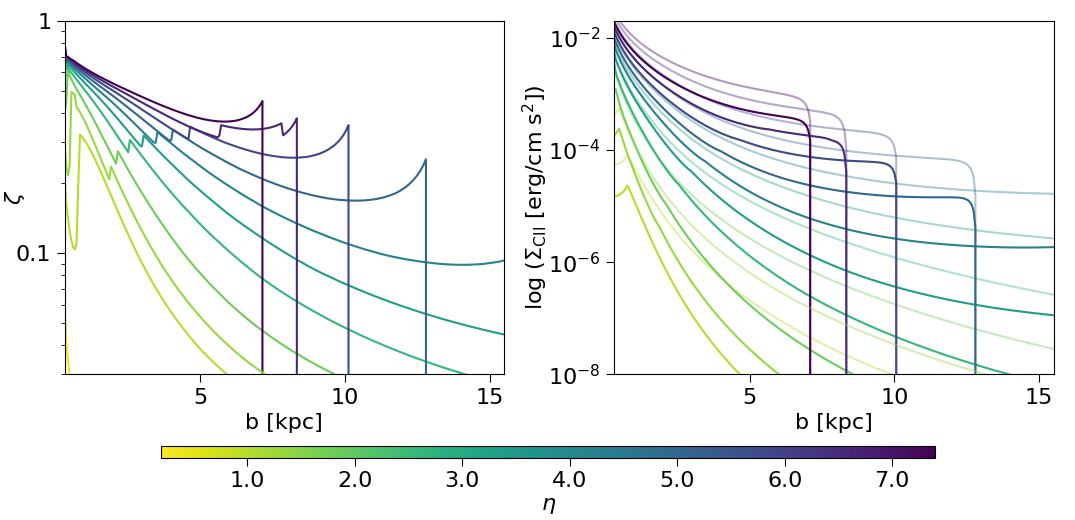
\includegraphics[width=1.0\textwidth]{plots/cmb_emission.png}
    \caption{\textit{Left}: suppression factor $\zeta$ as a function of the impact parameter $b$, for different values of the mass loading factor $\eta$. \textit{Right}: \CII surface density $\Sigma_\mathrm{CII}$, computed for $\zeta(r)$ showed in the left panel, as well as for $\zeta =1$ (transparent lines).
    \label{fig:global_emission_cmb}
    }
\end{figure*}





\subsection{Computing the final emission profiles}


In the last paragraphs, we have successfully computed the \CII surface density for our outflow model. Our final aim is to compare the results of our model with the observations of extended \CII emission reported in chapter \ref{chap:halos}. In order to do that, however, we need to convert the surface density into a flux per unit solid angle (or surface brightness), which is the quantity that is actually measured by observers (e.g., figure \ref{fig:fuji_data}). We do this by dividing $\Sigma_\mathrm{CII}$ by the observed \CII linewidth $\Delta\nu_\mathrm{obs}$:
\begin{align}
\Delta\nu_\mathrm{obs} = \frac{\Delta {\rm v}}{c} \frac{\nu_*}{1+z}\,,
\end{align}
where $\nu_*=1900\,\mathrm{GHz}$ is the rest-frame frequency of the \CII line, and $\Delta\mathrm{v}$ is the observed Full-Width Half Maximum (FWHM) of the line, which is commonly expressed as a velocity spread. Since the luminosity per unit frequency and per unit solid angle of the \CII line can be written as: 
\begin{align}
\frac{\d\mathrm{L}_\mathrm{CII}}{\d \Omega \, \Delta \nu_\mathrm{obs}} = \frac{\Sigma_\mathrm{CII}}{\Delta \nu_\mathrm{obs}}d_A^2\,,
\end{align}
the flux per unit solid angle is then:
\begin{align}
\frac{\d{\cal F}}{\d\Omega} = \frac{\Sigma_\mathrm{CII}}{\Delta \nu_\mathrm{obs}}\frac{d_A^2}{4\pi d_L^2 } = \frac{\Sigma_\mathrm{CII}}{4\pi\Delta \nu_\mathrm{obs}(1+z)^4}
\end{align}
In the left panel of figure \ref{fig:global_profiles}, we plot this quantity -- measured in $\mathrm{mJy\,arcsec}^{-2}$ -- for different values of the parameter $\eta$. Note that, in order to simulate the observed flux, we have to assume a value for the FWHM of the \CII line. In this section, for illustrative purposes, we choose to consider the observational data from the F19 study \citep{Fujimoto19} (i.e., a stacking of 18 normal, $z\approx 6$, star-forming galaxies). In the next chapter, we will focus on a more detailed comparison between our results and the body of observational data available to date. 

%The FWHM measured by F19 is:
%\begin{align}
%    \Delta\mathrm{v} = \mathrm{FWHM} = 296\pm40\, \kms
%\end{align}
There is one last obstacle, however, that prevents a fair comparison with observations: data from ALMA are naturally convolved with a beam (or PSF) that -- depending on the resolution -- can have important effects on the final \CII emission. For this reason, we convolve our profiles with the beam taken from the observational data. The 2-d convolution of a planar image $I(x,y)$ with a beam $b(x,y)$ is defined as: 
\begin{align}
    (I*b)(x,y)= \int \d x' \d y' \, I(x',y')\,b(x-x',y-y')
\end{align}
The ALMA beam is usually taken to be (approximately) a 2-d gaussian with a non-uniform variance. However, since we are working in a spherically symmetric fashion, we consider the average over the azimuthal angle for the beam, obtaining a radial profile $b(r)$. An instance of this profile is shown with a dashed grey line in figure \ref{fig:global_profiles} (right panel): the observational data refer to the F19 sample. 

It is interesting to note that, if the two functions $I(r)$ and $b(r)$ are both radially symmetric, then their convolution $(I*b)(r)$ can be expressed in terms of Bessel functions as \citep[see e.g.,][]{Baddour:09}:
\begin{align}
    (I*b)(r)= \frac{1}{2\pi}\,\int_0^\infty \d \rho \, \mathcal{H}_0[I](\rho)\, \mathcal{H}_0[b](\rho) \, J_0(\rho r),
\end{align}
where $J_0$ is the zeroth order Bessel function, and $\mathcal{H}_0$ stands for the (zeroth order) Hankel transform:
\begin{align}
    \mathcal{H}_0[f](r) = \int f(r)\,J_0(\rho r)\,r\,\d r
\end{align}
However, from a numerical perspective, it is more convenient to work in the general 2-d setting and to exploit the power of the Fast Fourier Transform algorithm (FFT). In fact, it can be easily proven that the Fourier transform of the convolution of two functions is equal to their product in the Fourier space. Therefore, the convolution operation can be expressed as ($\mathcal{F}$ is the 2-d Fourier transform):
\begin{align}
    (I*b)(x,y) = \mathcal{F}^{-1}\left[\mathcal{F}[I]\,\mathcal{F}[b]\right](x,y)
\end{align}
In the right panel of figure \ref{fig:global_profiles}, we plot the same profiles considered in the left panel, but we convolve them with the F19 beam (grey dashed line). The F19 data (figure \ref{fig:fuji_data}) are also shown for reference. The \CII emission that arises from our outflow model has a profile shape and an order of magnitude which is compatible with the observational data, for different values of the mass loading factor $\eta$. In particular, high values of $\eta$ ($\eta\approx 6-8$) reach the \CII luminosity that is required to account for observations, while lower values of $\eta$ seem to be disfavored by this comparison. 

Several different physical processes are playing a role in our model in shaping the final profiles and the global \CII luminosity. As expected, the resulting surface brightness (figure \ref{fig:global_emission}, left panel) is stronger for higher $\eta$. This is because a very mass-loaded wind has a greater initial density (eq. \ref{eq:bound_cc85_1}), and this results in a greater \CII emission as $\Sigma_\mathrm{CII}$ depends on the gas density squared (eq. \ref{eq:emissivity_CII}). On the other hand, mass-loaded winds have also a lower initial velocity and are much more affected by the halo's gravitational potential. As a result, the stalling radius $r_\mathrm{stop}$ has a strong dependence on $\eta$. For this reason, the resulting surface brightness for $\eta \approx 6-8$ has a sharp drop for distances close to $r_\mathrm{stop}$. 

In principle, this drop in emission hinders the emergence of a \CII halo on $10-\mathrm{kpc}$ scales. However, when convolving the surface brightness with the ALMA beam, this sharp feature is smoothed and significant \CII emission can be found even for $r>r_\mathrm{stop}$. This implies that different values of $\eta$ result in halos that, despite showing slightly different profiles, have similar global properties: e.g., an extension on $10-\mathrm{kpc}$ scales, a total \CII luminosity of $L_\mathrm{CII}\approx 10^9\,\mathrm{L}_\odot$, a total gas (carbon) mass in the halo of $M\approx 10^{10} \,\msun$ ($M_\mathrm{C}\approx 4\times10^6 \,\msun$). These properties are compatible both with observations and with our theoretical knowledge of the CGM of high-z galaxies. 

Note that the resulting emission does not agree very well with data at small distances ($r\lesssim 2\,\mathrm{kpc}$). The reason for this could be that we are considering only the $\CII$ emission arising from the external halo, and we are neglecting the contribution of the central ISM. Hence, the missing flux could be recovered by including the contribution of the central galaxy (which is quite difficult to model).

Overall, these preliminary results are very encouraging, and they suggest exploring further how our model compares with the data: we devote the next chapter to this task. 




\begin{figure*}
    \centering
    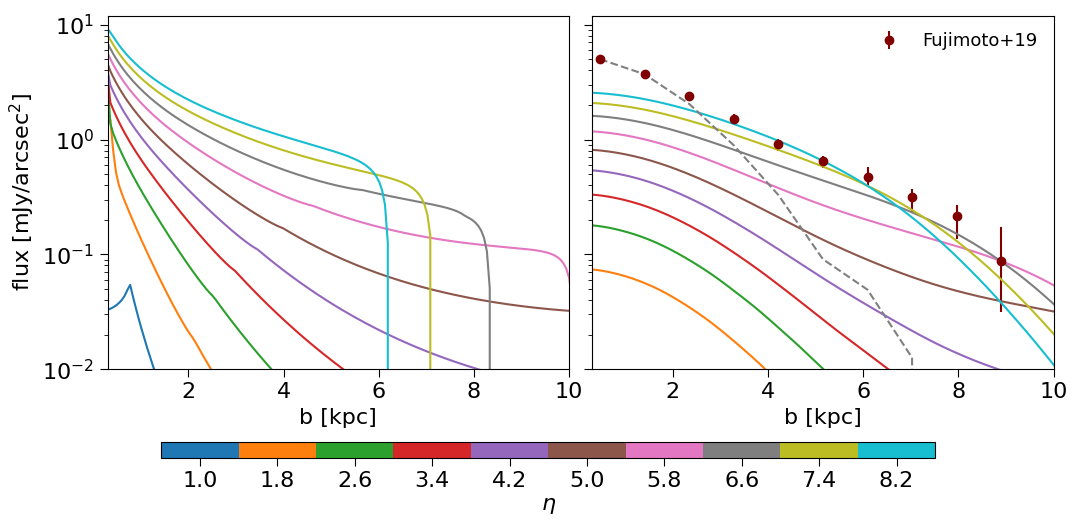
\includegraphics[width=1.0\textwidth]{plots/emission_final.png}
    \caption{\textit{Left}: \CII surface brightness profiles for different values of $\eta$ as a function of the impact parameter $b$. \textit{Right}: comparison of the profiles with data from F19 \citep{Fujimoto19}. The profiles are convolved with the same beam as in the observation (shown with a dashed grey line in the plot).
    \label{fig:global_emission}
    }
\end{figure*}






\begin{comment}


First, however, we briefly explore how these profiles are affected by different choices for our model parameters.


\subsection{Dependence on the halo circular velocity}\label{sec:vc_dependence}

COMMENT ON THE VC DEPENDENCE FURTHER; WHICH PLOTS TO SHOW HERE?


As a final step, we explore the dependence of the results on the dark matter halo circular velocity, $v_c$ (eq. \ref{eq:v_esc}).  We normalize the profiles to the central value of the F19 data to emphasize the differences in the profile shapes.


It is useful to comment on the dependence of \CII emission on $\eta$ and $v_c$. While $\eta$ affects primarily the overall halo brightness by regulating the outflow density, changing $v_c$ is equivalent to modify the strength of the gravitational field. As it is clear from Fig. \ref{fig:vesc_emission}, a deep gravitational potential ($v_c \gtrsim 200\kms$) results in values of $r_{\rm stop}$ which do not match the observed extension of the emitting halo. Weaker potentials ($v_c \simlt 150\kms$) are instead unable to slow down the outflow and therefore maintain a sufficiently high gas density in the outer regions of the halo. In this case, the low density of the gas results in a very faint (undetectable) emission. In addition, the low-density gas is more susceptible to photoionization by the galactic and/or cosmic UV field turning \CIIion into \CIIIion. Such a key role of the gravitational confinement has been noted also in recent hydrodynamical simulations results \citep{li2019supernovae}.


Generally, a tight anti-correlation between $\eta$ and $v_c$ is found, but the likelihood shows a narrow maximum around the values close to the ones identified previously, i.e. $\eta = 3.2 \pm 0.10$ (or $\dot{M}_\mathrm{out}= 128 \,\msun {\rm yr}^{-1}$) and $v_c = 170 \pm 10 \kms$. These results imply that extended halos might be used to set constrains on the mass loading factor and dark matter halo mass of early galaxies.


\begin{figure*}
    \centering
    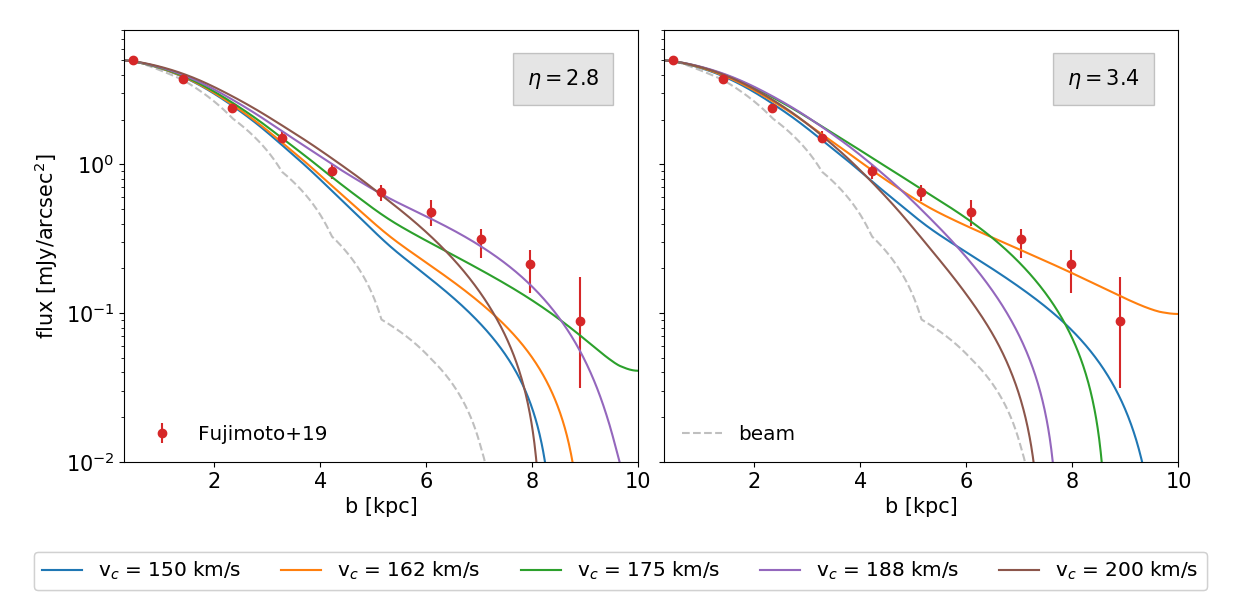
\includegraphics[width=1.025\textwidth,height=8.5cm]{vesc_emission_last.png}
    \caption{Predicted \CII surface brightness profiles (solid lines) as a function of the impact parameter $b$ for different values of the centrifugal velocity $v_\mathrm{c}$, compared with the data from F19 (points). Two values of the mass loading factor are shown: $\eta=2.8$ (left panel), $\eta=3.4$ (right). The profiles are normalised to the central value of the data, and convolved with the same ALMA beam (grey dashed line) used by F19.
    \label{fig:vesc_emission}
    }
\end{figure*}


\subsection{Dependence on metallicity}


 We have run new simulations of our model varying the gas metallicity. In particular, we have taken our best fit parameters ($\eta=3.2$ and $v_c=175$ km/s) and we have changed the metallicity between the two extreme values $Z=0.1, 1$. 
We find that, despite the fact that the cooling function significantly depends on metallicity, the final emission varies roughly linearly with $Z$, and this dependence in the emission is only due to carbon abundance in the gas. 
This is not unexpected, as the emission depends on gas density (and only marginally on gas temperature), on the CII ionization fraction, and on the carbon abundance (eq.s 17-18; NB: due to a typo, eq. 17 was missing an $A_C$ however correctly included in the calculations). Comparing the profiles for Z=0.1 and Z=1, we note that the density behaves similarly, while the temperature profiles are slightly different because of the different cooling functions; in both cases, though, the catastrophic cooling takes place within the first kpc. This means that CII ionization fraction is very similar in the two cases. Therefore, the only residual dependence of the CII emission is on the C abundance. Emission profiles normalized on the metallicity are thus quite similar in the two cases. 
Given this dependence, our best fit model provides a good fit for solar metallicity values. However, a higher mass loading factor and a lower circular velocity might accommodate metallicities as low as $Z=0.1$. Our choice of solar metallicity is motivated by both theoretical (numerical simulations at $z=6$, Pallottini+17,19) and empirical (extrapolation of the mass-metallicity relation for galaxies at $z=6$, Mannucci+12) arguments. 
We have added the corresponding text with this discussion in Sec. 3.2 of the paper. Here, for referee's convenience, we attach three plots: Figure \ref{fig:cooling} shows the cooling functions for the metallicities $Z=1$ and $Z=0.1$, Figure \ref{fig:ionization} shows the carbon ionization fraction in the two cases, and Figure \ref{fig:emission} the emission normalized on the metallicity.




\begin{figure}
	\centering
	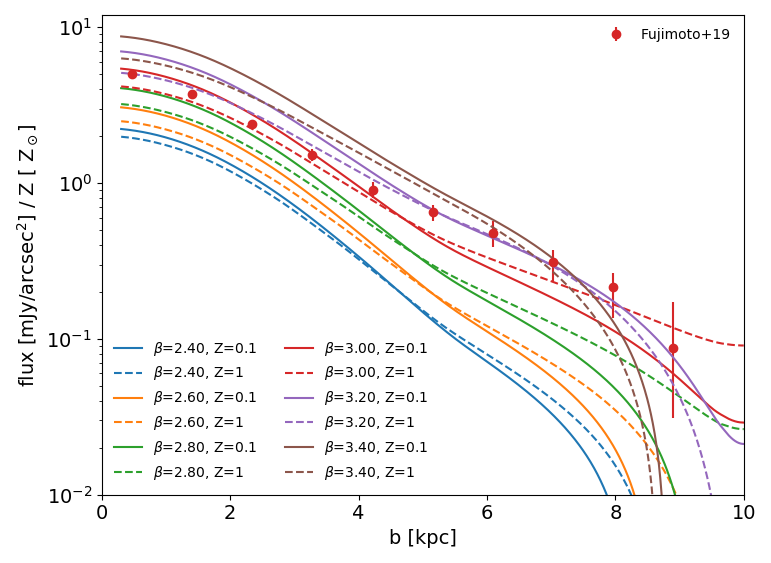
\includegraphics[width=0.8\textwidth]{plots/emission_Zeta_dependence.png}
	\caption{CII emission (as described in the right column of Figure 5 in the paper) for the two values of the metallicites $\mathrm{Z}=0.1$ (lefft) and $\mathrm{Z}=1$ (right). 
	}
	\label{fig:emission}
\end{figure}

\end{comment}



